\documentclass[12pt]{article}
\usepackage{graphicx}           
\usepackage{amsmath,amssymb}    
\usepackage{setspace}
\usepackage{tikz}
\usetikzlibrary{babel, quotes, angles}
\setlength{\parindent}{0pt}

\usepackage{listings}
\usepackage{xcolor}

\lstset{
    language=R,
    basicstyle=\ttfamily\small,
    keywordstyle=\bfseries\color{blue},
    commentstyle=\color{gray},
    stringstyle=\color{red},
    numbers=left,
    numberstyle=\tiny\color{gray},
    stepnumber=1,
    numbersep=10pt,
    backgroundcolor=\color{white},
    showspaces=false,
    showstringspaces=false,
    frame=single,
    tabsize=4,
    breaklines=true,
    breakatwhitespace=false,
    captionpos=b,
    keepspaces=true,
    escapeinside={\%*}{*)},
    morekeywords={*,...}
}


\title{\Huge Trabalho de Cálculo II}
\author{\Large Pablo Caballero Maciel}
\date{\large Agosto 2024}

\begin{document}
\maketitle
\newpage
\onehalfspacing

\tableofcontents

\section{Aproximações para PI}
\noindent Começaremos abordando alguns métodos geométricos para aproximações de PI. Por definição, adotaremos que \[\pi=\frac{C}{D}\] sendo C o comprimento da circunferência e D o diâmetro da mesma.
\vspace{0.2cm}\\
\noindent Em um primeiro momento, vamos criar um quadrado de lado L e inscrever uma circunferência de diâmetro D e comprimento C como a figura abaixo:
\vspace{0.1cm}

\begin{center}
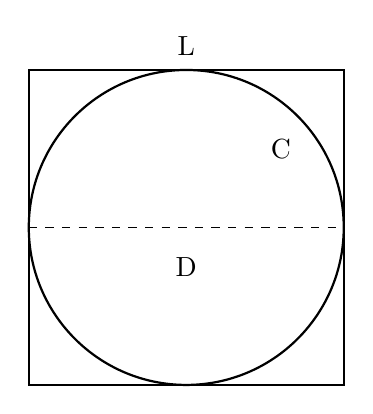
\begin{tikzpicture}
\def\L{4}
\def\D{4}
\draw[thick] (0,0) rectangle (\L, \L);
\draw[thick] (\L/2, \L/2) circle (\D/2);
\draw[dashed] (0, \L/2) -- (\L, \L/2);
    \node at (\L/2, \L+0.3) {L};
    \node at (\L/2, \L/2 - 0.5) {D};
    \node at (\D/2 + 1.2, \D/2 + 1 ) {C};
\end{tikzpicture}
\end{center}

\vspace{0.2cm} 
\noindent Dada a figura, podemos dizer que: \[2D<C<4L=4D \]  \[2<\frac{C}{D}<4 \] \[2<\pi<4 \]
\noindent Ou seja, o valor de PI está entre 2 e 4, o que ainda é algo muito vago.
\newpage
\noindent Desta vez vamos inserir um outro quadrado de lado l na figura: \\

\begin{center}
\begin{tikzpicture}
\def\L{4}
\def\D{4}
\draw[thick] (0,0) rectangle (\L, \L);
\draw[thick] (\L/2, \L/2) circle (\D/2);
\draw[thick] (\L/2-\D/2, \L/2) -- (\L/2, \L/2+\D/2) -- (\L/2+\D/2, \L/2) -- (\L/2, \L/2-\D/2) -- cycle;
    \node at (\D/2 + 1.3, \D/2 + 1 ) {l}
\draw[dashed] (0, \L/2) -- (\L, \L/2);
\draw[dashed] (\L/2, \L) -- (\L/2, 0);
    \node at (\L/2, \L+0.3) {L};
    \node at (\D/2 + 1.6, \D/2 + 1.6 ) {C};
\draw [thick, red](\L/2, \L/2) -- (\L/2, \L);
    \node at (\L/2 - 0.4, \L/2 + 0.7) {$\frac{D}{2}$};
\draw [thick, red](\L/2, \L/2) -- (\L, \L/2);
\draw [thick, red](\L, \L/2) -- (\L/2, \L);
\end{tikzpicture}
\end{center}

Assim, temos que: \[ 4l<C<4L=4D \] e por Teorema de Pitágoras temos que: \[l^{2}=2\left(\frac{L}{2}\right)^2=2\frac{L^2}{4}=\frac{D^2}{2}\Rightarrow l=\frac{D}{\sqrt{2}}=\frac{\sqrt{2}}{2}D\] Portanto: \[4\frac{\sqrt{2}}{2}D<C<4D\] 
          \[2\sqrt{2} < \frac{C}{D} < 4\]  
          \[2\sqrt{2} < \pi < 4\]
Isso nos deixa com um valor de PI que está entre aproximadamente 2,82 e 4. Ainda longe do desejado.
\newpage

Então vamos tentar fazer o mesmo mas dessa vez com um héxagono regular inscrito:

\begin{center}
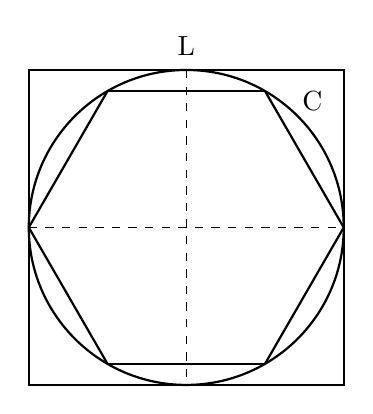
\begin{tikzpicture}
\def\L{4}
\def\D{4} 
\def\R{\D/2}

\draw[thick] (0,0) rectangle (\L, \L);

\draw[thick] (\L/2, \L/2) circle (\R);

\draw[dashed] (0, \L/2) -- (\L, \L/2);
\draw[dashed] (\L/2, \L) -- (\L/2, 0);

\foreach \i in {0,1,2,3,4,5} {
    \draw[thick] 
        ({\L/2 + \R * cos(60*\i)}, {\L/2 + \R * sin(60*\i)})
        -- ({\L/2 + \R * cos(60*(\i+1))}, {\L/2 + \R * sin(60*(\i+1))});
}

\node at (\L/2, \L+0.3) {L};
\node at (\D/2 + 1.6, \D/2 + 1.6) {C};
\end{tikzpicture}
\end{center}

Antes de começarmos o cálculo da aproximação, precisamos descobrir quanto vale o lado do hexágono. E, para isso, vamos desenhar um triângulo nele:

\begin{center}
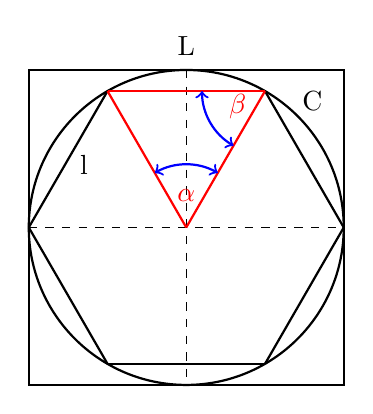
\begin{tikzpicture}
\def\L{4}
\def\D{4} 
\def\R{\D/2}

\draw[thick] (0,0) rectangle (\L, \L);

\draw[thick] (\L/2, \L/2) circle (\R);

\draw[dashed] (0, \L/2) -- (\L, \L/2);
\draw[dashed] (\L/2, \L) -- (\L/2, 0);

\foreach \i in {0,1,2,3,4,5} {
    \draw[thick] 
        ({\L/2 + \R * cos(60*\i)}, {\L/2 + \R * sin(60*\i)})
        -- ({\L/2 + \R * cos(60*(\i+1))}, {\L/2 + \R * sin(60*(\i+1))});
}

\node at (\L/2, \L+0.3) {L};
\node at (\D/2 + 1.6, \D/2 + 1.6) {C};
\node at (\L/2 - 1.3, \L/2 + 0.8) {l};

\draw[thick, red] (\L/2, \L/2) -- ({\L/2 + \R * cos(60)}, {\L/2 + \R * sin(60)});
\draw[thick, red] (\L/2, \L/2) -- ({\L/2 + \R * cos(120)}, {\L/2 + \R * sin(120)});
\draw[thick, red] ({\L/2 + \R * cos(60)}, {\L/2 + \R * sin(60)}) -- ({\L/2 + \R * cos(120)}, {\L/2 + \R * sin(120)});

\draw [step=.5cm, red, thick]
-- (\L/2, \L/2) coordinate (a)
-- ({\L/2 + \R * cos(60)}, {\L/2 + \R * sin(60)}) coordinate (b)
-- ({\L/2 + \R * cos(120)}, {\L/2 + \R * sin(120)}) coordinate (c)

pic["$\alpha$", draw=blue, <->, angle eccentricity=0.5, angle radius=0.8cm]{angle=b--a--c};


\draw [step=.5cm, red, thick]
-- (\L/2, \L/2) coordinate (a)
-- ({\L/2 + \R * cos(60)}, {\L/2 + \R * sin(60)}) coordinate (b)
-- ({\L/2 + \R * cos(120)}, {\L/2 + \R * sin(120)}) coordinate (c)

pic["$\beta$", draw=blue, <->, angle eccentricity=0.5, angle radius=0.8cm]{angle=c--b--a};
\end{tikzpicture}
\end{center}
Com isso, temos que: \[ 6\alpha=2\pi\Rightarrow\alpha=\frac{2\pi}{6}=\frac{\pi}{3}\] 
Por outro lado: \[2\beta=\pi-\alpha=\pi-\frac{\pi}{3}=\frac{2\pi}{3}\Rightarrow\beta=\frac{\pi}{3}\]
Portanto, como \[\alpha=\beta\]  o triângulo é equilátero e descobrimos que: \[ l=\frac{D}{2}\]
Agora vamos encontrar o lado no caso de a circunferência estiver inscrita ao hexágono:

\begin{center}
    
\tikzset{every picture/.style={line width=0.75pt}} %set default line width to 0.75pt        

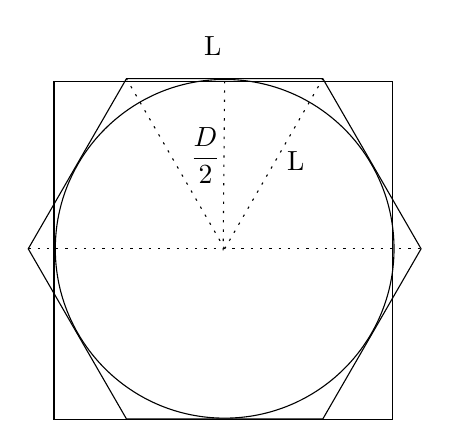
\begin{tikzpicture}[x=0.75pt,y=0.75pt,yscale=-1,xscale=1]
%uncomment if require: \path (0,300); %set diagram left start at 0, and has height of 300

%Shape: Square [id:dp18051493376115246] 
\draw   (273.41,52) -- (436.41,52) -- (436.41,215) -- (273.41,215) -- cycle ;
%Shape: Polygon [id:dp5195451557624688] 
\draw   (450.27,132.78) -- (402.95,214.73) -- (308.32,214.73) -- (261,132.78) -- (308.32,50.82) -- (402.95,50.82) -- cycle ;
%Shape: Ellipse [id:dp7810103236514105] 
\draw   (274.04,132.78) .. controls (274.04,87.71) and (310.57,51.19) .. (355.64,51.19) .. controls (400.7,51.19) and (437.23,87.71) .. (437.23,132.78) .. controls (437.23,177.84) and (400.7,214.37) .. (355.64,214.37) .. controls (310.57,214.37) and (274.04,177.84) .. (274.04,132.78) -- cycle ;
%Straight Lines [id:da7638384007494474] 
\draw  [dash pattern={on 0.84pt off 2.51pt}]  (261,132.78) -- (450.27,132.78) ;
%Straight Lines [id:da825071747390467] 
\draw  [dash pattern={on 0.84pt off 2.51pt}]  (354.91,133.5) -- (355.64,51.19) ;
%Straight Lines [id:da3881215203579953] 
\draw  [dash pattern={on 0.84pt off 2.51pt}]  (355.64,132.78) -- (308.32,50.82) ;
%Straight Lines [id:da48875841770013295] 
\draw  [dash pattern={on 0.84pt off 2.51pt}]  (355.64,132.78) -- (402.95,50.82) ;

% Text Node
\draw (353.67,35.24) node   [align=left] {\begin{minipage}[lt]{11.82pt}\setlength\topsep{0pt}
L
\end{minipage}};
% Text Node
\draw (393.67,90.58) node   [align=left] {\begin{minipage}[lt]{11.82pt}\setlength\topsep{0pt}
L
\end{minipage}};
\draw (348.67,80.58) node [align=left] {
        \begin{minipage}[lt]{11.82pt}
            \setlength\topsep{0pt}
            \[ \frac{D}{2} \]
        \end{minipage}
    };

\end{tikzpicture}
\end{center}
Deste modo: \[L^2=\left(\frac{D}{2}\right)^2+\left(\frac{L}{2}\right)^2=\frac{D^2}{4}+\frac{L^2}{4}\]  
E: \[\frac{3}{4}L^2=L^2(1-\frac{1}{4})=\frac{D^2}{4}\Rightarrow L=\frac{D}{\sqrt{3}}\]
Portanto, unindo os dois casos: \[6l<C<6L\] \[6\frac{D}{2}<C<6\frac{D}{\sqrt{3}}=\frac{2\cdot 3}{\sqrt{3}}D=2\sqrt3D\] \[3<\frac{C}{D}<2\sqrt3\] \[3<\pi<2\sqrt3\]
O  que revela um intervalo entre 3 e aproximadamente 3,46 para o valor de PI, um pouco melhor do que os anteriores.
\newpage
Se quando passamos a usar o hexágono no lugar do quadrado para aproximar o valor de PI nós obtivemos valores mais próximos, o que aconteceria se usássemos polígonos de mais lados?\\

Em 250 a.c, Arquimedes usou um polígono de 96 lados (16 vezes maior que o hexágono) e obteve:\[\pi\approx\frac{22}{7}=3,1428571\]\\
Em 265 d.c, Liu Hui usou um polígono de 3072 lados (512 vezes maior que o hexágono) e estimou:\[\frac{307}{98}<\pi<\frac{307}{99}\] \[3,1416<\pi<3,1427\]\\
Em 480 d.c, Zu Chongzhi usou um polígono de 12888 lados (2048 vezes maior que o hexágono) e calculou: \[\pi\approx\frac{355}{113}=3,1415929\]
\newpage
\subsection{Duplicação do quadrado}
Vamos fazer uma pausa para discutir sobre o problema da duplicação do quadrado.\\
Supondo que queremos duplicar um quadrado de lado L:

\begin{center}
    
\tikzset{every picture/.style={line width=0.75pt}} %set default line width to 0.75pt        

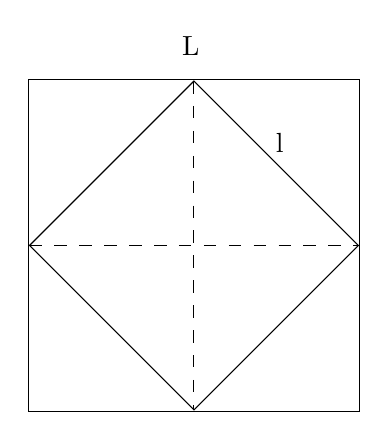
\begin{tikzpicture}[x=0.75pt,y=0.75pt,yscale=-1,xscale=1]
%uncomment if require: \path (0,300); %set diagram left start at 0, and has height of 300

%Shape: Square [id:dp18051493376115246] 
\draw   (271.67,51.33) -- (431.33,51.33) -- (431.33,211) -- (271.67,211) -- cycle ;
%Shape: Square [id:dp2193444721802955] 
\draw   (351.5,51.96) -- (430.71,131.17) -- (351.5,210.38) -- (272.29,131.17) -- cycle ;
%Straight Lines [id:da6606318216813152] 
\draw  [dash pattern={on 4.5pt off 4.5pt}]  (351.5,51.96) -- (351.5,131.17) -- (351.5,210.38) ;
%Straight Lines [id:da3671336344773237] 
\draw  [dash pattern={on 4.5pt off 4.5pt}]  (272.29,131.17) -- (351.5,131.17) -- (430.71,131.17) ;

% Text Node
\draw (353.67,35.24) node   [align=left] {\begin{minipage}[lt]{11.82pt}\setlength\topsep{0pt}
L
\end{minipage}};
% Text Node
\draw (398.87,81.64) node   [align=left] {\begin{minipage}[lt]{11.82pt}\setlength\topsep{0pt}
l
\end{minipage}};


\end{tikzpicture}
\end{center}
Pelo Teorema de Pitágoras: \[l^2=2\left(\frac{L}{2}\right)^2=2\frac{L^2}{4}\] \[2l^2=L^2\]
Mas será que isso está certo? vamos tentar provar!\\
Supondo um régua onde "u" seja a unidade de medição e "m" e "n" sejam números tais que: 
\[m\cdot u=L\]
\[n\cdot u=l\]

\begin{center}
    
\tikzset{every picture/.style={line width=0.75pt}} %set default line width to 0.75pt        

\begin{tikzpicture}[x=0.75pt,y=0.75pt,yscale=-1,xscale=1]
%uncomment if require: \path (0,300); %set diagram left start at 0, and has height of 300

%Shape: Rectangle [id:dp4179075706761495] 
\draw   (250.8,62.01) -- (602.63,62.01) -- (602.63,169.4) -- (250.8,169.4) -- cycle ;
%Straight Lines [id:da224404567304465] 
\draw    (283.3,60.6) -- (283.3,129.84) ;
%Straight Lines [id:da07371519713541064] 
\draw    (320.04,63.43) -- (320.04,94.51) ;
%Straight Lines [id:da17281633014379127] 
\draw    (352.54,62.01) -- (352.54,93.1) ;
%Straight Lines [id:da40811672262283194] 
\draw    (390.36,62.67) -- (390.36,93.75) ;
%Straight Lines [id:da4021070135371796] 
\draw    (426.01,61.9) -- (426.01,92.99) ;
%Straight Lines [id:da5147485204071429] 
\draw    (459.92,63.43) -- (459.92,94.51) ;
%Straight Lines [id:da6250469153936005] 
\draw    (496.44,62.67) -- (496.44,93.75) ;
%Straight Lines [id:da06526055963759014] 
\draw    (530.9,62.01) -- (530.9,93.1) ;
%Straight Lines [id:da31766685561716645] 
\draw    (564.48,63.43) -- (564.48,132.66) ;
%Shape: Brace [id:dp5962371995674518] 
\draw   (390.06,99.69) .. controls (390.06,104.36) and (392.39,106.69) .. (397.06,106.69) -- (397.33,106.69) .. controls (404,106.69) and (407.33,109.02) .. (407.33,113.69) .. controls (407.33,109.02) and (410.66,106.69) .. (417.33,106.69)(414.33,106.69) -- (417.6,106.69) .. controls (422.27,106.69) and (424.6,104.36) .. (424.6,99.69) ;

% Text Node
\draw (280.63,137.32) node [anchor=north west][inner sep=0.75pt]  [font=\tiny] [align=left] {0};
% Text Node
\draw (406.25,122.34) node [anchor=north west][inner sep=0.75pt]  [font=\tiny] [align=left] {u};


\end{tikzpicture}

\end{center}
\newpage
Resgatando o resultado do Teorema de Pitágoras: \[2=\frac{L^2}{l^2}=\frac{m^2\cdot u^2}{n^2\cdot u^2}=\left(\frac{m}{n}\right)^2\]
\textbf{\textit{Teorema:}} não existe nenhum número irracional tal que: \[r^2=2\]
\textbf{\textit{Demostração:}} por redução ao absurdo, suponha que: \[r=\frac{m}{n}\]
tal que: \[2=r^2=\frac{m^2}{n^2}\Rightarrow 2n=\frac{m^2}{n}\Rightarrow 2n-m=\frac{m^2}{n}-m\cdot\frac{n}{n}=\frac{m}{n}\left(m-n\right)\Rightarrow \] \[\Rightarrow\frac{2n-m}{m-n}=\frac{m}{n}\]
Agora, observe que:
\begin{center}
    

\tikzset{every picture/.style={line width=0.75pt}} %set default line width to 0.75pt        

\begin{tikzpicture}[x=0.75pt,y=0.75pt,yscale=-1,xscale=1]
%uncomment if require: \path (0,300); %set diagram left start at 0, and has height of 300

%Shape: Square [id:dp21773347043430147] 
\draw   (190.27,60.47) -- (414.4,60.47) -- (414.4,284.6) -- (190.27,284.6) -- cycle ;
%Shape: Square [id:dp1305845927763689] 
\draw   (302.33,61.13) -- (413.73,172.53) -- (302.33,283.93) -- (190.93,172.53) -- cycle ;
%Straight Lines [id:da13593142321106444] 
\draw  [dash pattern={on 0.84pt off 2.51pt}]  (302.33,61.13) -- (302.33,172.53) ;
%Straight Lines [id:da8831392614231686] 
\draw  [dash pattern={on 0.84pt off 2.51pt}]  (302.33,172.53) -- (413.73,172.53) ;

% Text Node
\draw (356.8,99.2) node [anchor=north west][inner sep=0.75pt]   [align=left] {n};
% Text Node
\draw (294.4,42.2) node [anchor=north west][inner sep=0.75pt]   [align=left] {m};

\draw (340.4,175.2) node [anchor=north west][inner sep=0.75pt]   [align=left] {$\frac{m}{2}$};
\end{tikzpicture}

\end{center}
\newpage
A partir disso: \[\frac{m}{2}<n\Rightarrow m<2n\] \[n<\frac{m}{2}+\frac{m}{2}=m\]
Portanto: \[2n-m>0 \]
\begin{center}
    e
\end{center} \[m-n>0 \]
são inteiros \textbf{positivos!} Além disso, tem-se que: \[n<m<2n\Rightarrow 0<m-n<n\]
\begin{center}
    e
\end{center}
\[n<m<2n\Rightarrow 2n<2m=m+m\Rightarrow 2n-m<m\]
Em suma: \[m,2n-m,\cdots \] é uma sequência estritamente decrescente de inteiros positivos, o que é um \textbf{absurdo!} \\

\textbf{\textit{Prova alternativa:}} Seja \[\left(\frac{m}{n}\right)^2=2\] e suponha, sem perda de generalidade, que "m" e "n" são coprimos, ou seja, (m,n) = 1.
\newpage
Agora, observe que: \[\frac{m^2}{n^2}=2\Rightarrow m^2=2n^2\]
"m" será par se: \[\left\{\begin{matrix}m=2k+1\Rightarrow m^2=4k^2+4k+1=2k\left(2k+2\right)+1.\hspace{0.3cm}\textbf{impar,\hspace{0.2cm}absurdo!}\\\hspace{-10.8cm}m=2k\hspace{0.2cm}\textbf{par}\end{matrix}\right.\]
Portanto: \[m^2=\left(2k\right)^2=4k^2=2n^2\Rightarrow n^2=2k^2\Rightarrow\textbf{n par}\]
Porém:
\[n=2k\hspace{0.2cm}e\hspace{0.2cm}m=2k\Rightarrow(m,n)\geq 2\hspace{0.2cm}\textbf{absurdo!}\]
\textbf{Corolário:} Ou a duplicação do quadrado é impossível (\textbf{falso}) ou existe em magnitudes incomensuráveis.
\subsection{Teorema do quadrado perfeito}
\textbf{Teorema:} Se "N" não é um quadrado perfeito, então \(\sqrt{N}\) é irracional\\
\textbf{Demonstração:} Se \(\sqrt{N} = \frac{m}{n}\), então:
\[N=\frac{m^2}{n^2}\Rightarrow m^2=N\cdot n^2=N\cdot n\cdot n\]
\[\frac{n}{m^2}=m\cdot m\Rightarrow\frac{n}{m}\hspace{0.3cm}se\hspace{0.3cm}(m,n)=1\]
Agora dado que obviamente \(\frac{n}{n}\) segue que \((m,n)\geq n\).\\
Portanto, é um \textbf{absurdo} ou n = 1, em cujo caso \(N=m^2\), sendo um quadrado perfeito.
\newpage
\subsection{Área do círculo}
Voltando às aproximações de PI, vamos usar a área do circulo para chegar nos resultados. Lembrando que adotamos PI como \(\pi=\frac{C}{D}\)\\
Em um primeiro momento, podemos dividir o círculo em quatro setores:
\begin{center}

    

\tikzset{every picture/.style={line width=0.75pt}} %set default line width to 0.75pt        

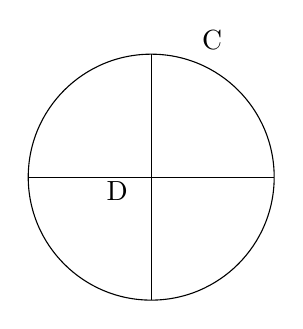
\begin{tikzpicture}[x=0.75pt,y=0.75pt,yscale=-1,xscale=1]
%uncomment if require: \path (0,300); %set diagram left start at 0, and has height of 300

%Shape: Circle [id:dp540788198774107] 
\draw   (211,98.75) .. controls (211,66.03) and (237.53,39.5) .. (270.25,39.5) .. controls (302.97,39.5) and (329.5,66.03) .. (329.5,98.75) .. controls (329.5,131.47) and (302.97,158) .. (270.25,158) .. controls (237.53,158) and (211,131.47) .. (211,98.75) -- cycle ;
%Straight Lines [id:da1079685492734781] 
\draw    (270.25,39.5) -- (270.25,158) ;
%Straight Lines [id:da8343642724476696] 
\draw    (211,98.75) -- (329.5,98.75) ;

% Text Node
\draw (293.5,27) node [anchor=north west][inner sep=0.75pt]   [align=left] {C};
% Text Node
\draw (247.5,99.5) node [anchor=north west][inner sep=0.75pt]   [align=left] {D};


\end{tikzpicture}
\end{center}
E vamos distribuir os setores de tal forma:
\begin{center}
    
\tikzset{every picture/.style={line width=0.75pt}} %set default line width to 0.75pt        

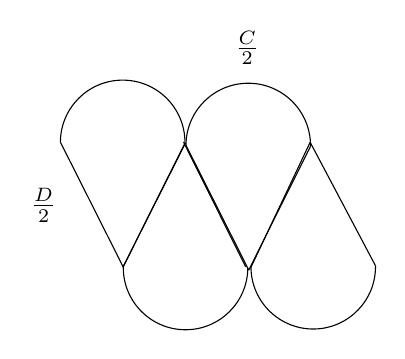
\begin{tikzpicture}[x=0.75pt,y=0.75pt,yscale=-1,xscale=1]
%uncomment if require: \path (0,300); %set diagram left start at 0, and has height of 300

%Shape: Arc [id:dp36382505387941877] 
\draw  [draw opacity=0] (140,60.4) .. controls (140.05,43.91) and (153.41,30.54) .. (169.92,30.5) .. controls (186.49,30.46) and (199.96,43.85) .. (200,60.42) .. controls (200,60.58) and (200,60.74) .. (200,60.9) -- (170,60.5) -- cycle ; \draw   (140,60.4) .. controls (140.05,43.91) and (153.41,30.54) .. (169.92,30.5) .. controls (186.49,30.46) and (199.96,43.85) .. (200,60.42) .. controls (200,60.58) and (200,60.74) .. (200,60.9) ;  
%Straight Lines [id:da5787591831452461] 
\draw    (140,60.4) -- (170.25,120.5) ;
%Straight Lines [id:da7308807714497607] 
\draw    (200,60.9) -- (170.25,120.5) ;
%Shape: Arc [id:dp16407527627412777] 
\draw  [draw opacity=0] (230.29,121) .. controls (230.17,137.49) and (216.75,150.8) .. (200.24,150.77) .. controls (183.67,150.75) and (170.26,137.3) .. (170.29,120.73) .. controls (170.29,120.57) and (170.29,120.41) .. (170.29,120.25) -- (200.29,120.77) -- cycle ; \draw   (230.29,121) .. controls (230.17,137.49) and (216.75,150.8) .. (200.24,150.77) .. controls (183.67,150.75) and (170.26,137.3) .. (170.29,120.73) .. controls (170.29,120.57) and (170.29,120.41) .. (170.29,120.25) ;  
%Straight Lines [id:da44362984573230557] 
\draw    (229.29,120.5) -- (199.29,60.27) ;
%Straight Lines [id:da15568643635619694] 
\draw    (170.29,120.25) -- (200.29,60.77) ;
%Shape: Arc [id:dp26485015015200175] 
\draw  [draw opacity=0] (200.5,61.9) .. controls (200.55,45.41) and (213.91,32.04) .. (230.42,32) .. controls (246.99,31.96) and (260.46,45.35) .. (260.5,61.92) .. controls (260.5,62.08) and (260.5,62.24) .. (260.5,62.4) -- (230.5,62) -- cycle ; \draw   (200.5,61.9) .. controls (200.55,45.41) and (213.91,32.04) .. (230.42,32) .. controls (246.99,31.96) and (260.46,45.35) .. (260.5,61.92) .. controls (260.5,62.08) and (260.5,62.24) .. (260.5,62.4) ;  
%Straight Lines [id:da7952232012323568] 
\draw    (200.5,61.9) -- (230.75,122) ;
%Straight Lines [id:da18589134876731395] 
\draw    (260.5,62.4) -- (230.75,122) ;
%Shape: Arc [id:dp9927923645918881] 
\draw  [draw opacity=0] (291.8,119.91) .. controls (292.09,136.39) and (279,150.03) .. (262.5,150.41) .. controls (245.93,150.79) and (232.2,137.67) .. (231.81,121.11) .. controls (231.81,120.95) and (231.81,120.79) .. (231.81,120.63) -- (261.81,120.42) -- cycle ; \draw   (291.8,119.91) .. controls (292.09,136.39) and (279,150.03) .. (262.5,150.41) .. controls (245.93,150.79) and (232.2,137.67) .. (231.81,121.11) .. controls (231.81,120.95) and (231.81,120.79) .. (231.81,120.63) ;  
%Straight Lines [id:da5239986610856924] 
\draw    (291.8,119.91) -- (260.33,60.44) ;
%Straight Lines [id:da7435909241187408] 
\draw    (231.81,120.63) -- (260.33,60.44) ;

% Text Node
\draw (223,5.5) node [anchor=north west][inner sep=0.75pt]   [align=left] {$\frac{C}{2}$};
% Text Node
\draw (124.5,81.5) node [anchor=north west][inner sep=0.75pt]   [align=left] {$\frac{D}{2}$};


\end{tikzpicture}

\end{center}
Tal que: \[ A\approx\frac{C}{2}\cdot\frac{D}{2}\]
Se dividirmos mais:
\begin{center}
    

\tikzset{every picture/.style={line width=0.75pt}} %set default line width to 0.75pt        

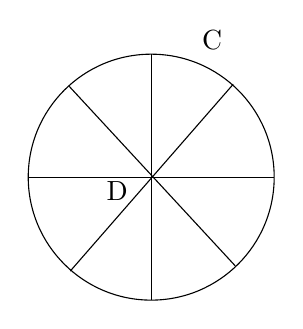
\begin{tikzpicture}[x=0.75pt,y=0.75pt,yscale=-1,xscale=1]
%uncomment if require: \path (0,300); %set diagram left start at 0, and has height of 300

%Shape: Circle [id:dp540788198774107] 
\draw   (211,98.75) .. controls (211,66.03) and (237.53,39.5) .. (270.25,39.5) .. controls (302.97,39.5) and (329.5,66.03) .. (329.5,98.75) .. controls (329.5,131.47) and (302.97,158) .. (270.25,158) .. controls (237.53,158) and (211,131.47) .. (211,98.75) -- cycle ;
%Straight Lines [id:da1079685492734781] 
\draw    (270.25,39.5) -- (270.25,158) ;
%Straight Lines [id:da8343642724476696] 
\draw    (211,98.75) -- (329.5,98.75) ;
%Straight Lines [id:da8560491422404692] 
\draw    (230.75,55) -- (310.75,141.5) ;
%Straight Lines [id:da6390688429135942] 
\draw    (309.75,54) -- (231.25,144) ;

% Text Node
\draw (293.5,27) node [anchor=north west][inner sep=0.75pt]   [align=left] {C};
% Text Node
\draw (247.5,99.5) node [anchor=north west][inner sep=0.75pt]   [align=left] {D};


\end{tikzpicture}

\end{center}
Ficamos com:
\begin{center}
    
\tikzset{every picture/.style={line width=0.75pt}} %set default line width to 0.75pt        

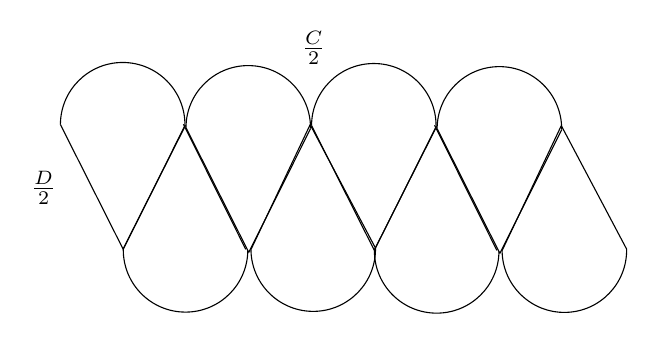
\begin{tikzpicture}[x=0.75pt,y=0.75pt,yscale=-1,xscale=1]
%uncomment if require: \path (0,300); %set diagram left start at 0, and has height of 300

%Shape: Arc [id:dp36382505387941877] 
\draw  [draw opacity=0] (140,60.4) .. controls (140.05,43.91) and (153.41,30.54) .. (169.92,30.5) .. controls (186.49,30.46) and (199.96,43.85) .. (200,60.42) .. controls (200,60.58) and (200,60.74) .. (200,60.9) -- (170,60.5) -- cycle ; \draw   (140,60.4) .. controls (140.05,43.91) and (153.41,30.54) .. (169.92,30.5) .. controls (186.49,30.46) and (199.96,43.85) .. (200,60.42) .. controls (200,60.58) and (200,60.74) .. (200,60.9) ;  
%Straight Lines [id:da5787591831452461] 
\draw    (140,60.4) -- (170.25,120.5) ;
%Straight Lines [id:da7308807714497607] 
\draw    (200,60.9) -- (170.25,120.5) ;
%Shape: Arc [id:dp16407527627412777] 
\draw  [draw opacity=0] (230.29,121) .. controls (230.17,137.49) and (216.75,150.8) .. (200.24,150.77) .. controls (183.67,150.75) and (170.26,137.3) .. (170.29,120.73) .. controls (170.29,120.57) and (170.29,120.41) .. (170.29,120.25) -- (200.29,120.77) -- cycle ; \draw   (230.29,121) .. controls (230.17,137.49) and (216.75,150.8) .. (200.24,150.77) .. controls (183.67,150.75) and (170.26,137.3) .. (170.29,120.73) .. controls (170.29,120.57) and (170.29,120.41) .. (170.29,120.25) ;  
%Straight Lines [id:da44362984573230557] 
\draw    (229.29,120.5) -- (199.29,60.27) ;
%Straight Lines [id:da15568643635619694] 
\draw    (170.29,120.25) -- (200.29,60.77) ;
%Shape: Arc [id:dp26485015015200175] 
\draw  [draw opacity=0] (200.5,61.9) .. controls (200.55,45.41) and (213.91,32.04) .. (230.42,32) .. controls (246.99,31.96) and (260.46,45.35) .. (260.5,61.92) .. controls (260.5,62.08) and (260.5,62.24) .. (260.5,62.4) -- (230.5,62) -- cycle ; \draw   (200.5,61.9) .. controls (200.55,45.41) and (213.91,32.04) .. (230.42,32) .. controls (246.99,31.96) and (260.46,45.35) .. (260.5,61.92) .. controls (260.5,62.08) and (260.5,62.24) .. (260.5,62.4) ;  
%Straight Lines [id:da7952232012323568] 
\draw    (200.5,61.9) -- (230.75,122) ;
%Straight Lines [id:da18589134876731395] 
\draw    (260.5,62.4) -- (230.75,122) ;
%Shape: Arc [id:dp9927923645918881] 
\draw  [draw opacity=0] (291.8,119.91) .. controls (292.09,136.39) and (279,150.03) .. (262.5,150.41) .. controls (245.93,150.79) and (232.2,137.67) .. (231.81,121.11) .. controls (231.81,120.95) and (231.81,120.79) .. (231.81,120.63) -- (261.81,120.42) -- cycle ; \draw   (291.8,119.91) .. controls (292.09,136.39) and (279,150.03) .. (262.5,150.41) .. controls (245.93,150.79) and (232.2,137.67) .. (231.81,121.11) .. controls (231.81,120.95) and (231.81,120.79) .. (231.81,120.63) ;  
%Straight Lines [id:da5239986610856924] 
\draw    (291.8,119.91) -- (260.33,60.44) ;
%Straight Lines [id:da7435909241187408] 
\draw    (231.81,120.63) -- (260.33,60.44) ;
%Shape: Arc [id:dp6351151650827591] 
\draw  [draw opacity=0] (261,60.9) .. controls (261.05,44.41) and (274.41,31.04) .. (290.92,31) .. controls (307.49,30.96) and (320.96,44.35) .. (321,60.92) .. controls (321,61.08) and (321,61.24) .. (321,61.4) -- (291,61) -- cycle ; \draw   (261,60.9) .. controls (261.05,44.41) and (274.41,31.04) .. (290.92,31) .. controls (307.49,30.96) and (320.96,44.35) .. (321,60.92) .. controls (321,61.08) and (321,61.24) .. (321,61.4) ;  
%Straight Lines [id:da9831765502861645] 
\draw    (261,60.9) -- (291.25,121) ;
%Straight Lines [id:da44809653403676397] 
\draw    (321,61.4) -- (291.25,121) ;
%Shape: Arc [id:dp5713386662610391] 
\draw  [draw opacity=0] (351.29,121.5) .. controls (351.17,137.99) and (337.75,151.3) .. (321.24,151.27) .. controls (304.67,151.25) and (291.26,137.8) .. (291.29,121.23) .. controls (291.29,121.07) and (291.29,120.91) .. (291.29,120.75) -- (321.29,121.27) -- cycle ; \draw   (351.29,121.5) .. controls (351.17,137.99) and (337.75,151.3) .. (321.24,151.27) .. controls (304.67,151.25) and (291.26,137.8) .. (291.29,121.23) .. controls (291.29,121.07) and (291.29,120.91) .. (291.29,120.75) ;  
%Straight Lines [id:da16695997597827028] 
\draw    (350.29,121) -- (320.29,60.77) ;
%Straight Lines [id:da5836422655691786] 
\draw    (291.29,120.75) -- (321.29,61.27) ;
%Shape: Arc [id:dp9681104756932553] 
\draw  [draw opacity=0] (321.5,62.4) .. controls (321.55,45.91) and (334.91,32.54) .. (351.42,32.5) .. controls (367.99,32.46) and (381.46,45.85) .. (381.5,62.42) .. controls (381.5,62.58) and (381.5,62.74) .. (381.5,62.9) -- (351.5,62.5) -- cycle ; \draw   (321.5,62.4) .. controls (321.55,45.91) and (334.91,32.54) .. (351.42,32.5) .. controls (367.99,32.46) and (381.46,45.85) .. (381.5,62.42) .. controls (381.5,62.58) and (381.5,62.74) .. (381.5,62.9) ;  
%Straight Lines [id:da44498527950279887] 
\draw    (321.5,62.4) -- (351.75,122.5) ;
%Straight Lines [id:da650537744494613] 
\draw    (381.5,62.9) -- (351.75,122.5) ;
%Shape: Arc [id:dp6637120836135821] 
\draw  [draw opacity=0] (412.8,120.41) .. controls (413.09,136.89) and (400,150.53) .. (383.5,150.91) .. controls (366.93,151.29) and (353.2,138.17) .. (352.81,121.61) .. controls (352.81,121.45) and (352.81,121.29) .. (352.81,121.13) -- (382.81,120.92) -- cycle ; \draw   (412.8,120.41) .. controls (413.09,136.89) and (400,150.53) .. (383.5,150.91) .. controls (366.93,151.29) and (353.2,138.17) .. (352.81,121.61) .. controls (352.81,121.45) and (352.81,121.29) .. (352.81,121.13) ;  
%Straight Lines [id:da6334870668590502] 
\draw    (412.8,120.41) -- (381.33,60.94) ;
%Straight Lines [id:da39447706156587037] 
\draw    (352.81,121.13) -- (381.33,60.94) ;

% Text Node
\draw (255,14) node [anchor=north west][inner sep=0.75pt]   [align=left] {$\frac{C}{2}$};
% Text Node
\draw (124.5,81.5) node [anchor=north west][inner sep=0.75pt]   [align=left] {$\frac{D}{2}$};


\end{tikzpicture}

\end{center}
E concluímos que: \[ A\approx\frac{C}{2}\cdot\frac{D}{2}\]

Se continuarmos com fatias menores, obteremos: \[ A=\frac{C}{2}\cdot\frac{D}{2}=\frac{C}{D}\cdot\frac{D^2}{4}=\pi\left(\frac{D}{2}\right)^2\]\\
\subsection{Área de hexágonos}
Agora vamos tentar usando a área de hexágonos:
\begin{center}
    

\tikzset{every picture/.style={line width=0.75pt}} %set default line width to 0.75pt        

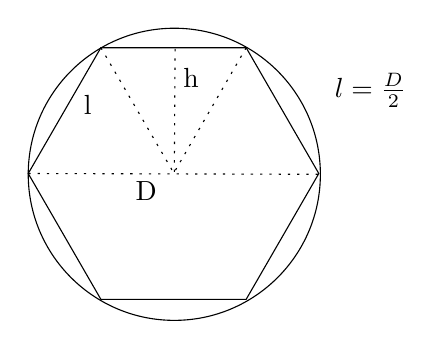
\begin{tikzpicture}[x=0.75pt,y=0.75pt,yscale=-1,xscale=1]
%uncomment if require: \path (0,300); %set diagram left start at 0, and has height of 300

%Shape: Circle [id:dp0016852678871273064] 
\draw   (189.5,109.38) .. controls (189.5,70.51) and (221.01,39) .. (259.88,39) .. controls (298.74,39) and (330.25,70.51) .. (330.25,109.38) .. controls (330.25,148.24) and (298.74,179.75) .. (259.88,179.75) .. controls (221.01,179.75) and (189.5,148.24) .. (189.5,109.38) -- cycle ;
%Shape: Regular Polygon [id:dp6965938202623108] 
\draw   (329.5,109) -- (294.5,169.62) -- (224.5,169.62) -- (189.5,109) -- (224.5,48.38) -- (294.5,48.38) -- cycle ;
%Straight Lines [id:da3792500890161079] 
\draw  [dash pattern={on 0.84pt off 2.51pt}]  (189.5,109) -- (330.25,109.38) ;
%Straight Lines [id:da23786936154379346] 
\draw  [dash pattern={on 0.84pt off 2.51pt}]  (260.25,49) -- (259.88,109.19) ;
%Straight Lines [id:da4658359461606394] 
\draw  [dash pattern={on 0.84pt off 2.51pt}]  (224.5,48.38) -- (259.88,109.19) ;
%Straight Lines [id:da4277085564529839] 
\draw  [dash pattern={on 0.84pt off 2.51pt}]  (294.5,48.38) -- (259.5,109) ;

% Text Node
\draw (263,57) node [anchor=north west][inner sep=0.75pt]   [align=left] {h};
% Text Node
\draw (240,111.5) node [anchor=north west][inner sep=0.75pt]   [align=left] {D};
% Text Node
\draw (336,59.5) node [anchor=north west][inner sep=0.75pt]   [align=left] {$l=\frac{D}{2}$};
\draw (215,70) node [anchor=north west][inner sep=0.75pt]   [align=left] {l};


\end{tikzpicture}

\end{center}
Desse modo: 
\[\left(\frac{D}{2}\right)^2=\left(\frac{l}{2}\right)^2+h^2\]
\[h^2=\frac{D^2}{4}-\frac{D^2}{4^2}=\frac{D^2}{4^2}(4-1)=\frac{3}{4^2}D^2\]
\[h=\frac{\sqrt3}{4}D\]
E, portanto:
\[6\cdot l\cdot h\cdot\frac{1}{2}=6\cdot\frac{D}{2}\cdot\frac{\sqrt3}{4}D\cdot\frac{1}{2}<\pi\frac{D^2}{4}\]
\[\frac{3\sqrt3}{2}<\pi\]\\
Por outro lado, se usarmos a circunferência inscrita ao hexágono:
\begin{center}
    

\tikzset{every picture/.style={line width=0.75pt}} %set default line width to 0.75pt        

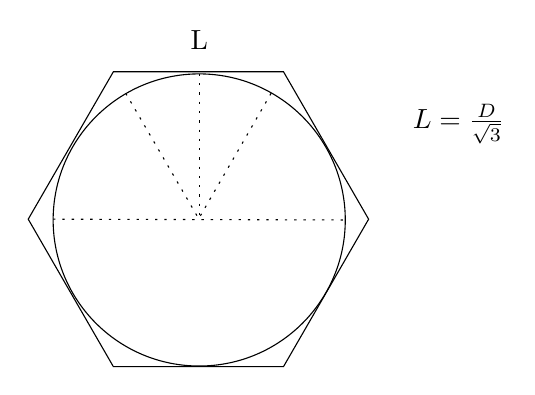
\begin{tikzpicture}[x=0.75pt,y=0.75pt,yscale=-1,xscale=1]
%uncomment if require: \path (0,300); %set diagram left start at 0, and has height of 300

%Shape: Circle [id:dp0016852678871273064] 
\draw   (189.5,109.38) .. controls (189.5,70.51) and (221.01,39) .. (259.88,39) .. controls (298.74,39) and (330.25,70.51) .. (330.25,109.38) .. controls (330.25,148.24) and (298.74,179.75) .. (259.88,179.75) .. controls (221.01,179.75) and (189.5,148.24) .. (189.5,109.38) -- cycle ;
%Shape: Regular Polygon [id:dp6965938202623108] 
\draw   (341.5,109) -- (300.5,180.01) -- (218.5,180.01) -- (177.5,109) -- (218.5,37.99) -- (300.5,37.99) -- cycle ;
%Straight Lines [id:da3792500890161079] 
\draw  [dash pattern={on 0.84pt off 2.51pt}]  (189.5,109) -- (330.25,109.38) ;
%Straight Lines [id:da23786936154379346] 
\draw  [dash pattern={on 0.84pt off 2.51pt}]  (259.88,39) -- (259.88,109.19) ;
%Straight Lines [id:da4658359461606394] 
\draw  [dash pattern={on 0.84pt off 2.51pt}]  (224.5,48.38) -- (259.88,109.19) ;
%Straight Lines [id:da4277085564529839] 
\draw  [dash pattern={on 0.84pt off 2.51pt}]  (294.5,48.38) -- (259.5,109) ;

% Text Node
\draw (254.5,17) node [anchor=north west][inner sep=0.75pt]   [align=left] {L};
% Text Node
\draw (361.5,52.5) node [anchor=north west][inner sep=0.75pt]   [align=left] {$L=\frac{D}{\sqrt3}$};


\end{tikzpicture}

\end{center}
Temos que:
\[\pi\cdot\frac{D^2}{4}<6\cdot L\cdot h\cdot\frac{1}{2}=6\cdot\frac{D}{\sqrt3}\cdot\frac{D}{2}\cdot\frac{1}{2}\]
\[\pi<\frac{6}{\sqrt3}=\frac{2\cdot 3}{\sqrt3}=\frac{2\cdot\sqrt3\cdot\sqrt3}{\sqrt3}=2\sqrt3\]
Concluindo que:
\[\frac{3\sqrt3}{2}<\pi<2\sqrt3\]
Ou seja, descobrimos que PI está entre aproximadamente 2,6 e 3,46
\newpage
\subsection{Papiro de Rhind}
O Papiro de Rhind, datado de 1550 a.C., é um dos mais antigos tratados matemáticos conhecidos, oferecendo uma visão detalhada sobre a matemática praticada no Antigo Egito. Escrito pelo escriba Ahmes, o documento abrange problemas que envolvem aritmética, álgebra simples e geometria.\footnote{Gillings, R. J. (1972). Mathematics in the Time of the Pharaohs. Dover Publications.}\vspace{0.5cm} \\
As técnicas que vamos ver a seguir foram utilizadas para calcular a área do círculo, mas que também resultou em uma aproximação de PI não intencional.\\
Comecemos com uma circunferência inscrita a um octógono:
\begin{center}
    



\tikzset{every picture/.style={line width=0.75pt}} %set default line width to 0.75pt        

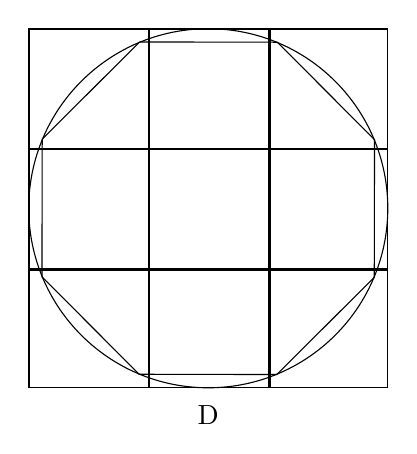
\begin{tikzpicture}[x=0.75pt,y=0.75pt,yscale=-1,xscale=1]
%uncomment if require: \path (0,300); %set diagram left start at 0, and has height of 300

%Shape: Square [id:dp06489624960251028] 
\draw   (203.88,44.88) -- (376.88,44.88) -- (376.88,217.88) -- (203.88,217.88) -- cycle ;
%Shape: Regular Polygon [id:dp16084392443610418] 
\draw   (323.4,211.49) -- (257.07,211.37) -- (210.26,164.4) -- (210.38,98.07) -- (257.35,51.26) -- (323.68,51.38) -- (370.49,98.35) -- (370.37,164.68) -- cycle ;
%Shape: Circle [id:dp7864553838925663] 
\draw   (203.88,131.38) .. controls (203.88,83.6) and (242.6,44.88) .. (290.38,44.88) .. controls (338.15,44.88) and (376.88,83.6) .. (376.88,131.38) .. controls (376.88,179.15) and (338.15,217.88) .. (290.38,217.88) .. controls (242.6,217.88) and (203.88,179.15) .. (203.88,131.38) -- cycle ;
%Shape: Grid [id:dp056530665590255325] 
\draw  [draw opacity=0][line width=0.75]  (203.88,44.88) -- (376.88,44.88) -- (376.88,217.88) -- (203.88,217.88) -- cycle ; \draw  [line width=0.75]  (203.88,44.88) -- (203.88,217.88)(261.88,44.88) -- (261.88,217.88)(319.88,44.88) -- (319.88,217.88) ; \draw  [line width=0.75]  (203.88,44.88) -- (376.88,44.88)(203.88,102.88) -- (376.88,102.88)(203.88,160.88) -- (376.88,160.88) ; \draw  [line width=0.75]   ;

% Text Node
\draw (284,225) node [anchor=north west][inner sep=0.75pt]   [align=left] {D};


\end{tikzpicture}


\end{center}
A partir disso, temos que:
\[A\approx\left(\frac{D^2}{3}\right)\cdot(9-2)=\frac{7}{9}D^2\]
Então:
\[\pi\frac{D^2}{4}=A\approx\frac{7}{9}D^2\]
\[\pi\approx\frac{28}{9}=3,\bar{1}\]
\newpage
Agora se pegarmos apenas um quadrante e dividirmos ele em 9:
\begin{center}
    

\tikzset{every picture/.style={line width=0.75pt}} %set default line width to 0.75pt        

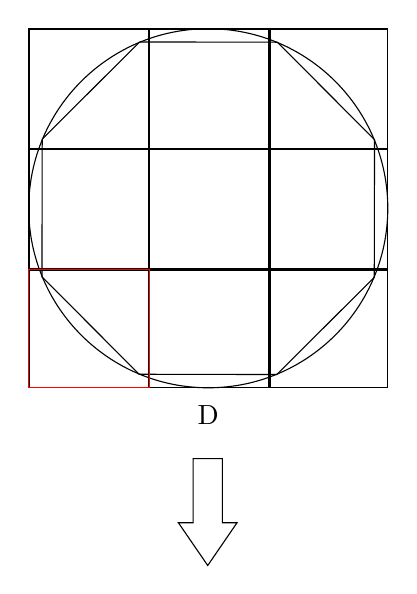
\begin{tikzpicture}[x=0.75pt,y=0.75pt,yscale=-1,xscale=1]
%uncomment if require: \path (0,300); %set diagram left start at 0, and has height of 300

%Shape: Square [id:dp06489624960251028] 
\draw   (202.38,2.38) -- (375.38,2.38) -- (375.38,175.38) -- (202.38,175.38) -- cycle ;
%Shape: Regular Polygon [id:dp16084392443610418] 
\draw   (321.9,168.99) -- (255.57,168.87) -- (208.76,121.9) -- (208.88,55.57) -- (255.85,8.76) -- (322.18,8.88) -- (368.99,55.85) -- (368.87,122.18) -- cycle ;
%Shape: Circle [id:dp7864553838925663] 
\draw   (202.38,88.88) .. controls (202.38,41.1) and (241.1,2.38) .. (288.88,2.38) .. controls (336.65,2.38) and (375.38,41.1) .. (375.38,88.88) .. controls (375.38,136.65) and (336.65,175.38) .. (288.88,175.38) .. controls (241.1,175.38) and (202.38,136.65) .. (202.38,88.88) -- cycle ;
%Shape: Grid [id:dp056530665590255325] 
\draw  [draw opacity=0][line width=0.75]  (202.38,2.38) -- (375.38,2.38) -- (375.38,175.38) -- (202.38,175.38) -- cycle ; \draw  [line width=0.75]  (202.38,2.38) -- (202.38,175.38)(260.38,2.38) -- (260.38,175.38)(318.38,2.38) -- (318.38,175.38) ; \draw  [line width=0.75]  (202.38,2.38) -- (375.38,2.38)(202.38,60.38) -- (375.38,60.38)(202.38,118.38) -- (375.38,118.38) ; \draw  [line width=0.75]   ;
%Straight Lines [id:da2163036488852046] 
\draw [color={rgb, 255:red, 255; green, 0; blue, 0 }  ,draw opacity=1 ]   (202.38,118.38) -- (260.38,118.38) ;
%Straight Lines [id:da19087932546078856] 
\draw [color={rgb, 255:red, 255; green, 0; blue, 0 }  ,draw opacity=1 ]   (202.38,175.38) -- (260.38,175.38) ;
%Straight Lines [id:da6022981699006782] 
\draw [color={rgb, 255:red, 255; green, 0; blue, 0 }  ,draw opacity=1 ]   (202.38,175.38) -- (202.38,118.38) ;
%Straight Lines [id:da7103426765894632] 
\draw [color={rgb, 255:red, 255; green, 0; blue, 0 }  ,draw opacity=1 ]   (260.38,175.38) -- (260.38,118.38) ;
%Right Arrow [id:dp18070143564125818] 
\draw   (295.69,209.5) -- (295.69,240.4) -- (302.75,240.4) -- (288.63,261) -- (274.5,240.4) -- (281.56,240.4) -- (281.56,209.5) -- cycle ;

% Text Node
\draw (282.5,182.5) node [anchor=north west][inner sep=0.75pt]   [align=left] {D};


\end{tikzpicture}

\end{center}
\begin{center}
    

\tikzset{every picture/.style={line width=0.75pt}} %set default line width to 0.75pt        

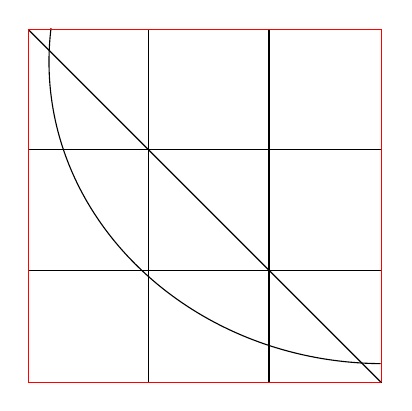
\begin{tikzpicture}[x=0.75pt,y=0.75pt,yscale=-1,xscale=1]
%uncomment if require: \path (0,300); %set diagram left start at 0, and has height of 300

%Shape: Square [id:dp5931621371378573] 
\draw  [color={rgb, 255:red, 0; green, 0; blue, 0 }  ,draw opacity=1 ] (199.25,40) -- (369.25,40) -- (369.25,210) -- (199.25,210) -- cycle ;
%Shape: Arc [id:dp49677366953129765] 
\draw  [draw opacity=0] (369.08,200.99) .. controls (280.68,200.31) and (209.25,135.43) .. (209.25,55.5) .. controls (209.25,50.05) and (209.58,44.68) .. (210.23,39.39) -- (370.5,55.5) -- cycle ; \draw   (369.08,200.99) .. controls (280.68,200.31) and (209.25,135.43) .. (209.25,55.5) .. controls (209.25,50.05) and (209.58,44.68) .. (210.23,39.39) ;  
%Shape: Grid [id:dp5258144589166414] 
\draw  [draw opacity=0] (199.25,40) -- (369.25,40) -- (369.25,210) -- (199.25,210) -- cycle ; \draw  [color={rgb, 255:red, 0; green, 0; blue, 0 }  ,draw opacity=1 ] (199.25,40) -- (199.25,210)(257.25,40) -- (257.25,210)(315.25,40) -- (315.25,210) ; \draw  [color={rgb, 255:red, 0; green, 0; blue, 0 }  ,draw opacity=1 ] (199.25,40) -- (369.25,40)(199.25,98) -- (369.25,98)(199.25,156) -- (369.25,156) ; \draw  [color={rgb, 255:red, 0; green, 0; blue, 0 }  ,draw opacity=1 ]  ;
%Straight Lines [id:da3177644422370973] 
\draw    (199.25,40) -- (369.25,210) ;
%Straight Lines [id:da9779275224425967] 
\draw [color={rgb, 255:red, 255; green, 0; blue, 0 }  ,draw opacity=1 ]   (199.25,40) -- (199.25,210) ;
%Straight Lines [id:da8626640216588857] 
\draw [color={rgb, 255:red, 255; green, 0; blue, 0 }  ,draw opacity=1 ]   (369.25,40) -- (369.25,210) ;
%Straight Lines [id:da5453797873705615] 
\draw [color={rgb, 255:red, 255; green, 0; blue, 0 }  ,draw opacity=1 ]   (199.25,40) -- (369.25,40) ;
%Straight Lines [id:da4517686963715595] 
\draw [color={rgb, 255:red, 255; green, 0; blue, 0 }  ,draw opacity=1 ]   (199.25,210) -- (369.25,210) ;




\end{tikzpicture}

\end{center}
Podemos ver que:
\[A\approx\left(\frac{D}{9}\right)^2\cdot(9^2-4\cdot\frac{9}{2})=\frac{D^2}{9^2}\cdot(9-2)\]
\[\frac{7}{9}D^2\]
Porém:
\[A\approx\left(\frac{D}{9}\right)^2\cdot(9^2-4\cdot\frac{9}{2})=\left(\frac{D}{9}^2\right)\cdot(81-18)\]
\[\left(\frac{D}{9}\right)^2\cdot 63\approx\left(\frac{D}{9}\right)^2\cdot 64 = \left(\frac{8}{9}D\right)^2 \]
\newpage
\subsubsection{Quadratura do círculo}
A partir disso, parece que a área do círculo tende a área do quadrado. Então, vamos verificar:
\[L^2=A=\frac{7}{9}D^2 \]
\[L=\sqrt{\frac{7}{9}}D\]
Por outro lado:
\[L^2=A=\left(\frac{8}{9}D\right)^2\]
\[L=\frac{8}{9}D\]
Por fim, obtemos como subproduto uma estimativa de PI:
\[\pi\cdot\frac{D^2}{4}=A=\left(\frac{8}{9}\right)^2\cdot D^2\]
\[\pi\approx\frac{4\cdot 8^2}{9^2}=\frac{2^8}{9^2}\]
\[\pi\approx\frac{256}{81}\approx 3,16\]
\newpage
\subsection{PI via Monte Carlo}
O método de Monte Carlo é uma técnica estatística que utiliza a geração de números aleatórios para resolver problemas matemáticos. Neste experimento, usaremos esse método para estimar o valor de \(\pi\). A ideia é gerar pontos aleatórios em um quadrado, verificar quantos caem dentro de um círculo inscrito, e usar essa proporção para calcular uma aproximação de \(\pi\). 

\subsubsection{Implementação em R}
\begin{lstlisting}[language=R, caption=Pi via Monte Carlo em R]
n = 100000
m = 1000
var = numeric(m)

for (i in 1:m) var[i] = single_shot(n)

single_shot = function(n) {
  x = runif(n)
  y = runif(n)
  z = x*x + y*y
  ins = which(z <= 1)
  pi = 4 * length(ins) / n
  return(pi)
}

plot(x[ins], y[ins], col='red', pch=19, cex=0.1, xlim=c(0,1), ylim=c(0,1))
points(x[-ins], y[-ins], col='blue', pch=19, cex=0.1)

mean(var)
sd(var) / sqrt(m)
\end{lstlisting}
\newpage
\begin{center}


\tikzset{every picture/.style={line width=0.75pt}} %set default line width to 0.75pt        

\begin{tikzpicture}[x=0.75pt,y=0.75pt,yscale=-1,xscale=1]
%uncomment if require: \path (0,300); %set diagram left start at 0, and has height of 300

%Shape: Axis 2D [id:dp4242630248212438] 
\draw  (331.31,246.78) -- (595.25,246.78)(357.71,23.95) -- (357.71,271.54) (588.25,241.78) -- (595.25,246.78) -- (588.25,251.78) (352.71,30.95) -- (357.71,23.95) -- (362.71,30.95)  ;
%Straight Lines [id:da6094387158492138] 
\draw  [dash pattern={on 0.84pt off 2.51pt}]  (367.37,59.53) -- (567.37,59.53) ;
%Straight Lines [id:da4980276059122324] 
\draw  [dash pattern={on 0.84pt off 2.51pt}]  (567.37,241.25) -- (567.37,59.53) ;
%Shape: Arc [id:dp6703242553974997] 
\draw  [draw opacity=0][dash pattern={on 0.84pt off 2.51pt}] (367.37,59.53) .. controls (422.09,69.16) and (476.22,99.59) .. (517.17,148.76) .. controls (540.42,176.68) and (556.97,207.69) .. (566.85,239.45) -- (360.66,279.11) -- cycle ; \draw  [dash pattern={on 0.84pt off 2.51pt}] (367.37,59.53) .. controls (422.09,69.16) and (476.22,99.59) .. (517.17,148.76) .. controls (540.42,176.68) and (556.97,207.69) .. (566.85,239.45) ;  
%Straight Lines [id:da273529987048037] 
\draw    (567.37,241.25) -- (567.37,252.79) ;
%Straight Lines [id:da07315320553515003] 
\draw  [dash pattern={on 0.84pt off 2.51pt}]  (366.89,193.18) -- (450.06,193.18) ;
%Straight Lines [id:da82603616144643] 
\draw  [dash pattern={on 0.84pt off 2.51pt}]  (450.06,240.29) -- (450.06,193.18) ;
%Shape: Ellipse [id:dp20923859310357518] 
\draw  [fill={rgb, 255:red, 0; green, 0; blue, 0 }  ,fill opacity=1 ] (452.56,193.18) .. controls (452.56,191.8) and (451.44,190.68) .. (450.06,190.68) .. controls (448.68,190.68) and (447.56,191.8) .. (447.56,193.18) .. controls (447.56,194.56) and (448.68,195.68) .. (450.06,195.68) .. controls (451.44,195.68) and (452.56,194.56) .. (452.56,193.18) -- cycle ;

% Text Node
\draw (565.23,257.87) node [anchor=north west][inner sep=0.75pt]  [font=\scriptsize] [align=left] {1};
% Text Node
\draw (347.93,188.64) node [anchor=north west][inner sep=0.75pt]  [font=\scriptsize] [align=left] {y};
% Text Node
\draw (447.93,251.14) node [anchor=north west][inner sep=0.75pt]  [font=\scriptsize] [align=left] {x};
% Text Node
\draw (346,253.06) node [anchor=north west][inner sep=0.75pt]  [font=\scriptsize] [align=left] {0};


\end{tikzpicture}

\end{center}
\begin{center}
    

\tikzset{every picture/.style={line width=0.75pt}} %set default line width to 0.75pt        

\begin{tikzpicture}[x=0.75pt,y=0.75pt,yscale=-1,xscale=1]
%uncomment if require: \path (0,299); %set diagram left start at 0, and has height of 299

%Image [id:dp8514412839919625] 
\draw (335.56,154.89) node  {\includegraphics[width=322.78pt,height=242.08pt]{Grafico_2.png}};




\end{tikzpicture}

\end{center}

\begin{center}
    

\tikzset{every picture/.style={line width=0.75pt}} %set default line width to 0.75pt        

\begin{tikzpicture}[x=0.75pt,y=0.75pt,yscale=-1,xscale=1]
%uncomment if require: \path (0,299); %set diagram left start at 0, and has height of 299

%Image [id:dp6815372882522328] 
\draw (326.83,150.25) node  {\includegraphics[width=312.5pt,height=234.38pt]{Grafico.png}};




\end{tikzpicture}

\end{center}

\subsubsection{Implementação em C}
\begin{lstlisting}[language=C, caption=Pi via Monte Carlo em C]
#include <stdio.h>
#include <stdlib.h>
#include <time.h>

int main(){
    double x, y;
    int n = 1000000;
    unsigned long long i, j;
    j = 0;
    srand(time(0));
    for (i = 1; i <= n; i++){
        x = (double)rand()/RAND_MAX;
        y = (double)rand()/RAND_MAX;
        if ((x*x + y*y) <= 1) j+=1;
    }
    double PI = 4*((double) j/n);
    printf("Valor de PI: %f", PI);
    return 0;
}
\end{lstlisting}

\subsubsection{Exercício: Determine o "valor médio" de \(\pi\). Interprete estatisticamente o resultado.}
Após realizar 100.000 simulações utilizando o método de Monte Carlo, o valor médio estimado de \(\pi\) foi 3,1416.\\
O valor médio de \(\pi\) obtido (3,1416) está muito próximo do valor real de \(\pi\) (3,14159), o que indica que o método de Monte Carlo é eficaz para estimar \(\pi\) com alta precisão. Além disso, o desvio padrão das estimativas foi baixo, refletindo que as simulações são consistentes e que a variabilidade das estimativas individuais de \(\pi\) é mínima. Isso reforça a confiabilidade da média calculada como uma boa aproximação do valor verdadeiro de \(\pi\).
\newpage
\section{Taylor via Série Geométrica}
Seja:\\
\(f(x)=-ln(1-x)\) \hspace{3cm} \(f(0)=-ln(1)=0\)\\ 
\(f'(x)=+(1-x)^{-1}\) \hspace{2.85cm} \(f'(0)=1\)\\ 
\(f''(x)=+(1-x)^{-2}\) \hspace{2.75cm} \(f''(0)=1\)\\
\(f'''(x)=+(1-x)^{-3}\) \hspace{2.65cm} \(f'''(0)=2\)\\
\(f^{4}(x)=+(1-x)^{-4}\) \hspace{2.7cm} \(f^{4}(0)=3!\)\\
\(\vdots\) \hspace{6.2cm} \(\vdots\)\\
\(f^{n}(x)=(n-1)!\cdot(1-x)^{-n}\) \hspace{1.2cm} \(f^{n}(0)=(n-1)!\)
\vspace{1cm}\\
Portanto:
\[-ln(1-x)=\sum_{n=0}^{\infty}\frac{f^{(n)}(0)}{n!}x^n=\sum_{n=1}^{\infty}\frac{(n-1)!}{n!}x^n\]
\[\sum_{n=1}^{\infty}\frac{x^n}{n}=\sum_{n=0}^{\infty}\frac{x^{n+1}}{n+1}\]
\textbf{\textit{Prova da convergência:}}
\[\frac{{a_{n}}+1}{{a\frac{}{}{n}}}=\frac{x^{n+1}}{n+1}\cdot\frac{n}{x^n}=\frac{n}{n+1}x\hspace{0.2cm},\hspace{0.3cm}tal\hspace{0.2cm}que\hspace{0.2cm}n+1<1\hspace{0.2cm}\forall n\in\mathbb{N}\]
Assim:
\[r=\displaystyle\lim_{n\to\infty}\left|\frac{{a_{n}}+1}{{a_{n}}}\right|=\left|x\right|\hspace{0.2cm},\hspace{0.1cm}se\hspace{0.1cm}\left|x\right|<1\]
Então:
\[-ln(1-x)=\sum_{n=1}^{\infty}\frac{x^n}{n}\hspace{0.2cm},\hspace{0.1cm}se\hspace{0.1cm}\left|x\right|<1\]
\begin{center}


\tikzset{every picture/.style={line width=0.75pt}} %set default line width to 0.75pt        

\begin{tikzpicture}[x=0.75pt,y=0.75pt,yscale=-1,xscale=1]
%uncomment if require: \path (0,299); %set diagram left start at 0, and has height of 299

%Shape: Axis 2D [id:dp13044074853933751] 
\draw  (189,131.28) -- (406.25,131.28)(213.44,27) -- (213.44,244.25) (399.25,126.28) -- (406.25,131.28) -- (399.25,136.28) (208.44,34) -- (213.44,27) -- (218.44,34)  ;
%Straight Lines [id:da9192830728796395] 
\draw    (259.06,128) -- (259.06,138) ;
%Straight Lines [id:da6064419380002739] 
\draw    (366.6,127) -- (366.6,131.68) -- (366.6,135.33) ;
%Curve Lines [id:da9882068443199712] 
\draw    (236.59,238.82) .. controls (244.19,145.4) and (255.05,83.49) .. (379.97,68.28) ;

% Text Node
\draw (212.93,120.44) node [anchor=north west][inner sep=0.75pt]   [align=left] {(};
% Text Node
\draw (360.23,120.77) node [anchor=north west][inner sep=0.75pt]   [align=left] {)};
% Text Node
\draw (254.45,139.33) node [anchor=north west][inner sep=0.75pt]  [font=\scriptsize] [align=left] {1};
% Text Node
\draw (362.57,136.17) node [anchor=north west][inner sep=0.75pt]  [font=\scriptsize] [align=left] {2};
% Text Node
\draw (204.83,132) node [anchor=north west][inner sep=0.75pt]  [font=\scriptsize] [align=left] {0};


\end{tikzpicture}


\end{center}
Em particular, se \(x=\frac{1}{2}\) tem-se:
\[0=ln(1)=ln\left(\frac{2}{2}\right)=ln\left(2\right)+ln\left(\frac{1}{2}\right)\]
\[ln(2)=-ln\left(\frac{1}{2}\right)=-ln\left(1-\frac{1}{2}\right)\]
\[\sum_{n=1}^{\infty}\frac{1}{2^n}\cdot\frac{1}{n}\]
Esta fórmula era conhecida por Jakob Bernoulli e serve para calcular os dígitos binários de \(ln(2)\), ou seja, em base 2.
\subsection{Exercício}
Analogamente, prove que:
\[ln(x+1)=-\sum_{k=1}^{\infty}\frac{(-x)^k}{k}=-\sum_{k=0}^{\infty}\frac{(-1)^{k+1}\cdot x^{k+1}}{(k+1)}=\sum_{k=0}^{\infty}(-1)^k\cdot\frac{x^{k+1}}{k+1}\]
Prove convergência no caso \(x=1\).
\newpage
\textbf{Resolução:}\\
\[\ln(1+x) = \sum_{k=1}^{\infty} \frac{(-1)^{k+1}}{k} x^k\]
Reescrevendo:
\[\ln(1+x) = -\sum_{k=1}^{\infty} \frac{(-x)^k}{k} \]

Expandindo os primeiros termos da série:

\[\ln(1+x) = x - \frac{x^2}{2} + \frac{x^3}{3} - \frac{x^4}{4} + \cdots \]

Por outro lado:

\[\sum_{k=1}^{\infty} \frac{(-x)^k}{k} = -\left( x - \frac{x^2}{2} + \frac{x^3}{3} - \frac{x^4}{4} + \cdots \right)\]

Portanto:

\[\ln(1+x) = -\sum_{k=1}^{\infty} \frac{(-x)^k}{k}\]
\newpage
\textbf{Prova da convergência:}

\[ \ln(2) = \sum_{k=1}^{\infty} \frac{(-1)^{k+1}}{k} \]

Pelo Teste de Leibniz, se os termos de uma série alternada diminuem monotonamente para zero, a série converge.

Portanto:

\[ \ln(1+x) = \sum_{k=1}^{\infty} \frac{(-1)^{k+1}}{k} x^k \]

converge para ( x = 1 ):

\[ \ln(2) = \sum_{k=1}^{\infty} \frac{(-1)^{k+1}}{k} \]
\newpage
\subsection{Série Geométrica de razão a:}
\[S_{n}=1+a+a^2+\cdots+a^{n}\]
\hspace{3cm} \(-\) \hspace{0.5cm} \(a\cdot S_{n}=a+a^2+\cdots+a^{n}+a^{n+1}\)

\vspace{-0.8cm}
\begin{center}\(\)
    
\tikzset{every picture/.style={line width=0.75pt}} %set default line width to 0.75pt        

\begin{tikzpicture}[x=0.75pt,y=0.75pt,yscale=-1,xscale=1]
%uncomment if require: \path (0,299); %set diagram left start at 0, and has height of 299

%Straight Lines [id:da10675470320753844] 
\draw    (185.5,71) -- (420.75,71) ;

\end{tikzpicture}

\end{center}
\vspace{-0.6cm}
\[S_n-aS_n=1-a^{n+1}\]
\[(1-a)S_n=1-a^{n+1}\]
\[S_n=\frac{1-a^{n+1}}{1-a}=\frac{1}{1-a}-\frac{a^{n+1}}{1-a}\]
Portanto:
\[\frac{1}{1-a}=S_n+\frac{a^{n+1}}{1-a}=\sum_{k=0}^{n}a^k+\frac{a^{n+1}}{1-a}\]
\[\underbrace{\frac{1}{1-x}}=\sum_{k=0}^{n}\underbrace{x^k}+\frac{x^{n+1}}{1-x}\]
\hspace{4.5cm} \large{\(f'(x)\)} \hspace{0.4cm} \Large{\(\left(\frac{x^{k+1}}{k+1}\right)'\)}\\
\normalsize{Então:}
\[-ln(1-x)=\sum_{k=0}^{n}\frac{x^{k+1}}{k+1}=\sum_{k=1}^{n+1}\frac{x^k}{k}\hspace{0.2cm}?\]
\textbf{\textit{Teorema:}} \(P_{n+1}(x)=\sum_{k=0}^{n}\frac{x^{k+1}}{k+1}\) é o polinômio de Taylor da função \(-ln(1-x)\) na origem.\\

\textbf{\textit{Demonstração:}}
\[0 = \displaystyle\lim_{x\to 0}\frac{-ln(1-x)-P_{n+1}(x)}{x^{n+1}}\xrightarrow[]{L'H\hat{o}pital}\displaystyle\lim_{x\to 0}\frac{x^{n+1}}{1-x}\cdot\frac{1}{(n+1)x^n}=\]

\[=\frac{1}{n+1}\cdot\displaystyle\lim_{x\to 0}\frac{1}{1-x}=0.\]

\[\frac{1}{1-x}=\sum_{k=0}^{n}x^k+\frac{x^{n+1}}{1-x}\]
Trocando \(x\) por \(-x^2\):
\[\underbrace{\frac{1}{1+x^2}}=\sum_{k=0}^{n}(-1)^k\cdot\underbrace{x^2k}+\frac{(-1)^{n+1}}{1+x^2}\cdot x^{2n+2}\]
\hspace{2.7cm} \large{\(arctg'(x)\)} \hspace{1.1cm} \Large{\(\left(\frac{x^{2k+1}}{2k+1}\right)'\)}
\vspace{1cm}\\
\normalsize{\textbf{\textit{Teorema:}}} \(P_{2n+1}(x)=\sum_{k=0}^{n}(-1)^k\cdot\frac{x^{2k+1}}{2k+1}\) é o polinomio de Taylor da função \(arctg(x)\) de ordem \(2n+1\) na origem.\\

Analogamente:
\[\frac{1}{1+x}=\sum_{k=0}^{n}(-1)^k+\frac{(-x)^{n+1}}{1+x}=\]
\[=\sum_{k=0}^{n}(-1)^k x^k+(-1)^{n+1}\cdot\frac{x^{n+1}}{1+x}\]
Portanto:
\[ln(1+x)=\underbrace{\sum_{k=0}^{n}(-1)^k\cdot\frac{x^{k+1}}{k+1}}+R_{n+1}(x)\]
\hspace{6.5cm} \(P_{n+1}\)\\
\[\frac{R_{n+1}(x)+R_{n+1}(0)}{x-0}=\frac{R_{n+1}(x)}{x}=R'_{n+1}(\xi)=(-1)^{n+1}\cdot\frac{\xi^{n+1}}{1+x}\hspace{0.2cm},\hspace{0.1cm}\xi\in(0,x)\]
Assim:
\[\left|R_{n+1}(x)\right|=\left|x\right|\cdot\frac{\left|\xi\right|^{n+1}}{\left|1+x\right|}<\left|x\right|\cdot\left|\xi\right|\underbrace{\leqslant}\left|\xi\right|^{n+1}\]
\hspace{8.4cm} \(0<x\leq 1\)\\
\section{Leibniz Aprimorado}
\[ arctg(x)=\underbrace{\sum_{k=0}^{n}(-1)^k\cdot\frac{x^{2k+1}}{2k+1}}+R_n(x)\hspace{0.2cm};\hspace{0.2cm}\left|R_n(x)\right|\leq\frac{x^{2n+3}}{2n+3}\]
\hspace{4.7cm} \(P_n(x)\)\\
\[arctg(x)=x-\frac{x^3}{3}+\frac{x^5}{5}-\frac{x^7}{7}+\frac{x^9}{9}-\frac{x^11}{11}+\cdots \]
\[\frac{\pi}{4}=arctg(1)=\left(1-\frac{1}{3}\right)+\left(\frac{1}{5}-\frac{1}{7}\right)+\left(\frac{1}{9}-\frac{1}{11}\right)+\cdots\left(\frac{1}{2n+1}-\frac{1}{2n+3}\right)\]
\vspace{0.1cm}\\
Como \(n=2k\) :
\[\frac{1}{2(2k)+1}-\frac{1}{2(2k)+3}=\frac{1}{4k+1}-\frac{1}{4k+3}\]
Então:
\[\frac{\pi}{4}=\sum_{k=0}^{\infty}\left(\frac{1}{4k+1}-\frac{1}{4k+3}\right)=\sum_{k=0}^{\infty}\frac{4k+3-4k-1}{(4k+1)(4k+3)}\]
\[\pi=8\cdot\sum_{k=0}^{\infty}\frac{1}{(4k+1)(4k+3)}\]
\newpage
Sabe-se que \(ln(1+x)=\sum_{k=0}^{\infty}(-1)^k\cdot\frac{x^{k+1}}{k+1}=x-\frac{x^2}{2}+\frac{x^3}{3}-\frac{x^4}{4}+\cdots\)
\vspace{0.2cm}\\
E também que:
\[\sum_{k=0}^{\infty}\frac{cos(k\pi)}{k+1}=\sum_{k=0}^{\infty}\frac{(-1)^k}{k+1}=ln(1+1)=ln(2).\]
E:
\[\sum_{k=0}^{\infty}\frac{sen(\frac{k\pi}{2})}{k+1}=\sum_{k=0}^{\infty}\frac{sen(2k+1)\cdot\frac{\pi}{2}}{(2k+1)+1}.\]
\[=\frac{1}{2}\cdot\sum_{k=0}^{\infty}\frac{sen(k\pi)\cdot cos(\frac{\pi}{2})+cos(k\pi)\cdot sen(\frac{\pi}{2})}{k+1}\]
\[=\frac{1}{2}\cdot\sum_{k=0}^{\infty}\frac{(-1)^k}{k+1}=\frac{1}{2}\cdot ln(1+1)=\frac{1}{2}\cdot ln(2)\]
Portanto:
\[\sum_{k=0}^{\infty}\frac{cos(k\pi)-2sen(\frac{k\pi}{2})}{k+1}=0\]
\textbf{\textit{Teorema:}} \(\sum_{k=0}^{\infty}\frac{a(k)}{k+1}=0\) ; onde \(a(k)=cos(k\pi)-2sen(\frac{k\pi}{2})\)
\vspace{0.5cm}\\
Agora, observe que: \(n=4k+r\), \(0\leq r < 4\).\\
Assim:
\[cos(n\pi)=cos(4k+r)\pi=cos(4k\pi)\cdot cos(r\pi)-sen(4k\pi)\cdot sen(r\pi)\]
\[=(-1)^r\]
E:
\[sen(\frac{n\pi}{2})=sen(4k+r)\frac{\pi}{2}=sen(2k\pi)\cdot cos(r\cdot\frac{\pi}{2})+cos(2k\pi)\cdot sen(r\cdot\frac{\pi}{2})\]
\[=sen(r\cdot\frac{\pi}{2})\left\{\begin{matrix}0\hspace{0.4cm}se\hspace{0.2cm}r=0\\1\hspace{0.4cm}se\hspace{0.2cm}r=1\\0\hspace{0.4cm}se\hspace{0.2cm}r=2\\-1\hspace{0.4cm}se\hspace{0.2cm}r=3\\\end{matrix}\right.\]
Portanto:
\[a(k)=cos(k\pi)-2sen(k\cdot\frac{\pi}{2})\]
\[=(-1)^k-2\left\{0,1,0,-1\right\}\hspace{0.2cm}mod\hspace{0.2cm}4\]
\[=\left\{1,-1,1,-1\right\}-2\left\{0,1,0,-1\right\}\hspace{0.2cm}mod\hspace{0.2cm}4\]
\[=\left\{1,-3,1,1\right\}\hspace{0.2cm}mod\hspace{0.2cm}4\]
Então:
\[0=\sum_{k=0}^{\infty}\left(\frac{1}{4k+1}-\frac{3}{4k+2}+\frac{1}{4k+3}+\frac{1}{4k+4}\right)\]
\hspace{1.8cm} \(+\)
\hspace{0.2cm}\Large{\(\frac{\pi}{4}=\sum_{k=0}^{\infty}\left(\frac{1}{4k+1}-\frac{1}{4k+3}\right)\)}
\begin{center}
    
\tikzset{every picture/.style={line width=0.75pt}} %set default line width to 0.75pt        

\begin{tikzpicture}[x=0.75pt,y=0.75pt,yscale=-1,xscale=1]
%uncomment if require: \path (0,299); %set diagram left start at 0, and has height of 299

%Straight Lines [id:da10675470320753844]
\draw    (110.5,40) -- (420.75,40) ;

\end{tikzpicture}

\end{center}

\hspace{2.5cm} \(\frac{\pi}{4}=\sum_{k=0}^{\infty}\left ( \frac{2}{4k+1}-\frac{3}{4k+2}+\frac{1}{4k+4}\right)\)
\newpage
\normalsize{}
Continuando:
\[
\frac{2}{4k+1} - \frac{3}{4k+2} + \frac{1}{4k+4} = \frac{A}{(4k+1)\cdot2(2k+1)\cdot4(k+1)}
\]
\[A=4^2\cdot(2k+1)(k+1)-3\cdot4(4k+1)(k+1)+2(4k+1)(2k+1)\]
\[
A = 4^{2} \left( 2k^2 + 3k + 1 \right) - 3 \cdot 4 \left( 4k^{2} + 5k + 1 \right) + 2\left(8k^{2} - 6k + 1 \right)
\]
\[
= k^{2} \left( 2 \cdot 16 - 3 \cdot 16 + 16 \right) = 0
\]
\[
+ k\left(3 \cdot 16 - 3 \cdot 20 + 3 \cdot 4\right) = 0
\]
\[
+ 16 - 12 + 2 = 6
\]
Portanto:
\[
\pi = \frac{4 \cdot 6}{2 \cdot 4} \sum_{k=0}^{\infty} \frac{1}{(4k+1)(2k+1)(k+1)}
\]
Alternativamente:
\[
\pi = 24 \sum_{k=0}^{\infty} \frac{1}{(4k+1)(4k+2)(4k+4)} 
\]
Adotando \((4k+1)(4k+2)(4k+4)\) como \((i+1)(i+2)(i+4)\) temos que:
\[
(i+1)(i+2)(i+4) = (i+1)(i+2)(i+2+2)\] 
\[= (i+1)\left[(i+2)^{2} + 2(i+2)\right]
\]
\[
= (i+1)\left[(i+1)^2+2(i+1)+ 1 + 2(i+1) + 2\right]
\]
\[
= (i+1)\left[(i+1)^{2} + 4(i+1) + 3\right]\] 
\[= (i+1)\left[(i+1)\left\{(i+1)+4\right\} + 3\right]
\]
\newpage
Além disso:
\[(k+a)(k+b)=k^2+(a+b)k+ab\]
Então:
\[(k+a)(k+b)(k+c)=k^3+ck^2+(a+b)k^2+(a+b)ck+abk+abc\]
\[=k^3+(a+b+c)k^2+(ab+ac+bc)k+abc\]
\[\frac{1}{k+1}-\frac{3}{k+2}=\frac{k+2-3k-3}{(k+1)(k+2)}=\frac{-(2k+1)}{(k+1)(k+2)}\]
Assim:
\[\frac{1}{k+1}-\frac{3}{k+2}+\frac{1}{k+4}=\frac{-(2k+1)(k+4)+k^2+3k+2}{(k+1)(k+2)(k+4)}\]
\[=\frac{-2k^2-9k-4+k^2+3k+2}{(k+1)(k+2)(k+4)}=\frac{-k^2-6k-2}{(k+1)(k+2)(k+4)}\]
Desse modo:
\[\frac{1}{k+1}-\frac{3}{k+2}+\frac{1}{k+4}+\frac{1}{k+3}=\frac{-(k^2+6k+2)(k+3)+k^3+7k^2+14k+8}{(k+1)(k+2)(k+3)(k+4)}\]
\[=\frac{-k^3-9k^2-20k-6+k^3+7k^2+14k+8}{\prod_{i=1}^{4}(k+i)}\]
\[=\frac{-2k^2-6k+2}{\prod_{i=1}^{4}(k+i)}=\frac{-2(k^2+3k-1)}{(k+1)(k+2)(k+3)(k+4)}\]
Pegando a equação quadrática:
\[k^2+3k-1=0\Leftrightarrow k=\frac{-3\pm\sqrt{9+4}}{2}=\frac{-3\pm\sqrt13}{2}\]
\[b(k)=\frac{1}{k+1}-\frac{3}{k+2}+\frac{1}{k+3}+\frac{1}{k+4}\]
E, portanto:
\[b(k)<0\hspace{0.7cm}\forall k\geq 1.\]
\[b(0)=\frac{2}{24}=\frac{1}{12}\hspace{0.2cm};\hspace{0.2cm}b(1)=\frac{-6}{24\cdot5}=-\frac{1}{20}\]
\begin{center}
    


\tikzset{every picture/.style={line width=0.75pt}} %set default line width to 0.75pt        

\begin{tikzpicture}[x=0.75pt,y=0.75pt,yscale=-1,xscale=1]
%uncomment if require: \path (0,299); %set diagram left start at 0, and has height of 299

%Shape: Axis 2D [id:dp23941725361098265] 
\draw  (203.21,161.54) -- (534.67,161.54)(362.92,6.5) -- (362.92,284.5) (527.67,156.54) -- (534.67,161.54) -- (527.67,166.54) (357.92,13.5) -- (362.92,6.5) -- (367.92,13.5)  ;
%Straight Lines [id:da1258103138093134] 
\draw    (323.27,154.19) -- (323.27,168.89) ;
%Straight Lines [id:da2422333607645455] 
\draw    (242.63,153.74) -- (242.63,168.44) ;
%Shape: Ellipse [id:dp9849452345490892] 
\draw  [fill={rgb, 255:red, 0; green, 0; blue, 0 }  ,fill opacity=1 ] (213.23,161.32) .. controls (213.23,159.59) and (214.63,158.2) .. (216.35,158.2) .. controls (218.07,158.2) and (219.47,159.59) .. (219.47,161.32) .. controls (219.47,163.04) and (218.07,164.43) .. (216.35,164.43) .. controls (214.63,164.43) and (213.23,163.04) .. (213.23,161.32) -- cycle ;
%Shape: Circle [id:dp16724460235776895] 
\draw  [fill={rgb, 255:red, 0; green, 0; blue, 0 }  ,fill opacity=1 ] (359.8,132.36) .. controls (359.8,130.64) and (361.2,129.24) .. (362.92,129.24) .. controls (364.65,129.24) and (366.04,130.64) .. (366.04,132.36) .. controls (366.04,134.08) and (364.65,135.48) .. (362.92,135.48) .. controls (361.2,135.48) and (359.8,134.08) .. (359.8,132.36) -- cycle ;
%Shape: Ellipse [id:dp3677205504178769] 
\draw  [fill={rgb, 255:red, 0; green, 0; blue, 0 }  ,fill opacity=1 ] (382.53,161.32) .. controls (382.53,159.59) and (383.92,158.2) .. (385.64,158.2) .. controls (387.37,158.2) and (388.76,159.59) .. (388.76,161.32) .. controls (388.76,163.04) and (387.37,164.43) .. (385.64,164.43) .. controls (383.92,164.43) and (382.53,163.04) .. (382.53,161.32) -- cycle ;
%Straight Lines [id:da23188926002135357] 
\draw    (402.57,153.74) -- (402.57,168.44) ;
%Curve Lines [id:da8766189473696857] 
\draw  [dash pattern={on 0.84pt off 2.51pt}]  (193.18,223.69) .. controls (232.83,72.21) and (340.65,38.8) .. (419.06,223.24) ;
%Shape: Ellipse [id:dp16690170208769328] 
\draw  [fill={rgb, 255:red, 0; green, 0; blue, 0 }  ,fill opacity=1 ] (400.35,187.6) .. controls (400.35,186.37) and (401.34,185.37) .. (402.57,185.37) .. controls (403.8,185.37) and (404.8,186.37) .. (404.8,187.6) .. controls (404.8,188.83) and (403.8,189.83) .. (402.57,189.83) .. controls (401.34,189.83) and (400.35,188.83) .. (400.35,187.6) -- cycle ;
%Straight Lines [id:da09617085547138782] 
\draw  [dash pattern={on 0.84pt off 2.51pt}]  (385.64,161.32) -- (385.64,217.45) ;
%Straight Lines [id:da8473915792605711] 
\draw  [dash pattern={on 0.84pt off 2.51pt}]  (385.64,217.45) -- (362.92,217.45) ;
%Straight Lines [id:da47325172279598604] 
\draw  [dash pattern={on 0.84pt off 2.51pt}]  (402.57,187.6) -- (362.92,187.6) ;
%Straight Lines [id:da28219570840245756] 
\draw  [dash pattern={on 0.84pt off 2.51pt}]  (402.57,161.76) -- (402.57,187.6) ;

% Text Node
\draw (235.58,172.97) node [anchor=north west][inner sep=0.75pt]  [font=\scriptsize] [align=left] {\mbox{-}3};
% Text Node
\draw (315.77,173.86) node [anchor=north west][inner sep=0.75pt]  [font=\scriptsize] [align=left] {\mbox{-}1};
% Text Node
\draw (353.19,164.5) node [anchor=north west][inner sep=0.75pt]  [font=\scriptsize] [align=left] {0};
% Text Node
\draw (191.2,140) node [anchor=north west][inner sep=0.75pt]  [font=\scriptsize] [align=left] {\mbox{-}3,3};
% Text Node
\draw (403.53,172.08) node [anchor=north west][inner sep=0.75pt]  [font=\scriptsize] [align=left] {1};
% Text Node
\draw (387.17,133.76) node [anchor=north west][inner sep=0.75pt]  [font=\scriptsize] [align=left] {0,3};


\end{tikzpicture}

\end{center}
\section{Fórmula de Machin}
\[\frac{\pi}{6}=arctg\left(\frac{1}{\sqrt3}\right)=\frac{1}{\sqrt3}\sum_{k=0}^{\infty}(-1)^k\cdot\frac{1}{3^k(2k+1)}+R_n\left(\frac{1}{\sqrt3}\right)\]
\[\left|R_n\right|\leq\frac{1}{\sqrt3}\cdot\frac{1}{3^{n+1}}\cdot\frac{1}{2n+3}\]
\[arctg(x)=\sum_{k=0}^{\infty}\frac{x^{4k+1}}{4k+1}-\frac{x^{4k+3}}{4k+3}=x^{4k+1}\left(\frac{1}{4k+1}-\frac{x^2}{4k+3}\right)\]
Portanto:
\[\frac{\pi}{6}=arctg\left(\frac{1}{\sqrt3}\right)=\frac{1}{\sqrt3}\sum_{k=0}^{\infty}\frac{1}{3^{2k}}\cdot\frac{12k+9-4k-1}{3(4k+1)(4k+3)}\]
\[\pi=\frac{6\cdot4}{\sqrt3\cdot3}\sum_{k=0}^{\infty}\frac{1}{3^{2k}}\cdot\frac{2k+2}{(2(2k)+1)(2(2k)+3)}\]
\[\pi=\frac{8\sqrt3}{3}\sum_{k=0}^{\infty}\frac{1}{3^i}\cdot\frac{i+2}{(2i+1)(2i+3)}\hspace{0.2cm},\hspace{0.2cm}i=i+2\]\\
\vspace{0.5cm}\textbf{\textit{Tratamento do erro:}} \(2(m+1)=2m+2<2m+3\Rightarrow \frac{1}{2m+3}<\frac{1}{2(m+1)}\)
Assim:
\[6R_n\leq\frac{6}{2n+3}\cdot\frac{1}{\sqrt3}\cdot\frac{1}{3^{n+1}}<\frac{6}{2(n+1)}\cdot\frac{1}{\sqrt3}\cdot\frac{1}{3^{n+1}}<\varepsilon\hspace{0.2cm}?\]
Então:
\[\frac{1}{\varepsilon}\cdot\frac{6}{2\sqrt3}<3^{n+1}(n+1)\]
\[=\frac{1}{\varepsilon}\cdot\sqrt3\]\\
\vspace{0.5cm}
\textbf{\textit{Tratamento do erro no caso geral:}}
\[A\cdot arctg\left(\frac{1}{a}\right)=A\cdot P_n\left(\frac{1}{a}\right)+A\cdot R_n\left(\frac{1}{a}\right)\]
\[=A\sum_{k=0}^{m}(-1)^k\cdot\frac{\left(\frac{1}{a}\right)^{2k+1}}{2k+1}+A\cdot R_n\left(\frac{1}{a}\right)\hspace{0.2cm},\hspace{0.2cm}\left|R_n\right|\leq\frac{\left(\frac{1}{a}\right)^{2m+3}}{2m+3}\]
Seguindo:
\[A\cdot\frac{1}{a^{2m+3}}\cdot\frac{1}{2m+3}<\frac{1}{a^{2m+3}}\cdot\frac{1}{2(m+1)}<\frac{\varepsilon}{q}\hspace{0.2cm}?\]
\[\frac{1}{\varepsilon}\cdot\frac{qA}{2a}<a^{2(m+1)}\cdot(m+1)\]
Se \(\varepsilon =10^{-d}\) tem-se:
\[10^d\cdot\frac{qA}{2a}<a^{2(m+1)}\cdot(m+1)\]

\subsection{Exercício:}
Integrando por partes, tem-se:
\[\int arctg(x)dx=x\cdot arctg(x)-\frac{1}{2}\cdot\int\frac{2x}{1+x^2}dx=x\cdot arctg(x)-\frac{1}{2}\cdot ln(1+x^2)\]
Então:
\[\frac{\pi}{4}=\int_{0}^{1}arctg(x)dx+\frac{1}{2}\cdot ln(2)\]
Agora:
\[\int_{0}^{1}arctg(x)dx=\sum_{k=0}^{\infty}(-1)^k\cdot\int_{0}^{1}\frac{x^{2k+1}}{2k+1}\]
\[=\sum_{k=0}^{\infty}(-1)^k\cdot\frac{1}{(2k+1)(2k+2)}\]
\[=\sum_{k=0}^{\infty}(-1)^k\cdot\left[\frac{1}{(2k+1)}-\frac{1}{2k+2}\right]\]
Por outro lado:
\[ln(1+x)=\sum_{k-0}^{\infty}(-1)^k\cdot\frac{x^{k+1}}{k+1}\hspace{0.2cm},\hspace{0.2cm}-1<x\leq 1\hspace{0.2cm}\Rightarrow \]
\[\Rightarrow ln(2)=ln(1+1)=\sum_{k=0}^{\infty}\frac{(-1)^k}{k+1}=\sum_{k=0}^{\infty}\left[\frac{1}{2k+1}-\frac{1}{2k+2}\right]\]
E:
\[\frac{\pi}{4}=\sum_{k=0}^{\infty}(1+\frac{1}{2})\cdot\left[\frac{1}{4k+1}-\frac{1}{4k+2}\right]+(-1+\frac{1}{2})\cdot\left[\frac{1}{4k+3}-\frac{1}{4k+4}\right]\]
Portanto:
\[\pi=2\cdot\sum_{k=0}^{\infty}\left[\frac{3}{4k+1}-\frac{3}{4k+2}-\frac{1}{4k+3}+\frac{1}{4k+4}\right]\]
\subsection{Exercício:}
Sejam \(a>0\)\hspace{0.2cm}e\hspace{0.2cm}\(0<\varepsilon<a^2\).\\
Prove que \(min(a-\sqrt{a^2-\varepsilon}, \sqrt{a^2-\varepsilon}-a) = \sqrt{a^2-\varepsilon}-a\)\\
\textbf{\textit{Demonstração:}}
Observe que:
\[(a^2-\varepsilon)(a^2+\varepsilon)=a^4-\varepsilon^2<a^4\Rightarrow \]
\[\Rightarrow\sqrt{a^2-\varepsilon}\cdot\sqrt{a^2+\varepsilon}<a^2\]
\[ 2\cdot\sqrt{a^2-\varepsilon}\cdot\sqrt{a^2+\varepsilon}<2a^2\]
\[ 2\cdot\sqrt{a^2-\varepsilon}\cdot\sqrt{a^2+\varepsilon}+\underbrace{2a^2}<2a^2+2a^2=4a^2=(2a)^2\]
\hspace{5.9cm}\(a^2+a^2=(a^2+\varepsilon)+(a^2-\varepsilon)\)\\
Assim:
\[(a^2+\varepsilon)+2\cdot\sqrt{a^2-\varepsilon}\cdot\sqrt{a^2+\varepsilon}+(a^2-\varepsilon)<(2a)^2\]

\[\left(\sqrt{a^2-\varepsilon}+\sqrt{a^2+\varepsilon}\right)^2<(2a)^2\]
\[\sqrt{a^2-\varepsilon}+\sqrt{a^2+\varepsilon}\underbrace{<}(2a)=a+a\hspace{0.2cm}(\ast)\]
\hspace{6.5cm} se\hspace{0.2cm}\(a>0\)\\
Portanto:
\[\sqrt{a^2+\varepsilon}-a<a-\sqrt{a^2-\varepsilon}\]
\newpage
\textbf{\textit{O/F:}} 
\[\ast\Rightarrow 1<\frac{2a}{\sqrt{a^2+\varepsilon}+\sqrt{a^2-\varepsilon}}\Rightarrow \]
\[\Rightarrow 1-\frac{2a}{\sqrt{a^2+\varepsilon}+\sqrt{a^2-\varepsilon}}<0\Rightarrow \]\\
\vspace{0.5cm}
\hspace{7.2cm} \footnotesize{\(=\varepsilon+\varepsilon=a^2+\varepsilon-a^2+\varepsilon=(a^2+\varepsilon)-(a^2-\varepsilon)\)}
\normalsize{}
\vspace{-0.8cm}\\
\[\Rightarrow-2\varepsilon+\frac{2a\cdot\overbrace{2\varepsilon}}{\sqrt{a^2+\varepsilon}+\sqrt{a^2-\varepsilon}}>0\]
\[-2\varepsilon+2a\cdot\frac{(a^2+\varepsilon)-(a^2-\varepsilon)}{\sqrt{a^2+\varepsilon}+\sqrt{a^2-\varepsilon}}>0\]
\[-2\varepsilon+2a\cdot\frac{(\sqrt{a^2+\varepsilon}-\sqrt{a^2-\varepsilon})(\sqrt{a^2+\varepsilon}+\sqrt{a^2-\varepsilon})}{\sqrt{a^2+\varepsilon}+\sqrt{a^2-\varepsilon}}>0\]
\[-2\varepsilon+2a\cdot(\sqrt{a^2+\varepsilon}-\sqrt{a^2-\varepsilon})>0\]
Então:
\[0<2a\sqrt{a^2+\varepsilon}-2a\sqrt{a^2-\varepsilon}\underbrace{-\varepsilon+2a^2-2a^2-\varepsilon}\]
\hspace{7cm} \((a^2-\varepsilon)+a^2-(a^2+\varepsilon)-a^2\)\\
\[=2a\sqrt{a^2+\varepsilon}-(a^2+\varepsilon)-a^2+(a^2-\varepsilon)-2a\sqrt{a^2-\varepsilon}+a^2\]
\[=(\sqrt{a^2-\varepsilon}-a)^2-(\sqrt{a^2+\varepsilon}-a)^2\]
\[=(\underbrace{a-\sqrt{a^2-\varepsilon}})^2-(\underbrace{\sqrt{a^2+\varepsilon}-a})^2\]
\hspace{5cm} \(=:\delta_1 \)\hspace{2.2cm} \(=:\delta_2 \)\\
Portanto:
\[\delta_1^2-\delta_2^2>0 \hspace{0.2cm}(\ast)\]
\newpage
Por outro lado, tem-se:
\[a^2-\varepsilon<a^2\Rightarrow\sqrt{a^2-\varepsilon}<a\Rightarrow 0<a-\sqrt{a^2-\varepsilon}=\delta_1\]
E, analogamente:
\[a^2+\varepsilon>a^2\Rightarrow\sqrt{a^2+\varepsilon}>a\Rightarrow 0<\sqrt{a^2+\varepsilon}-a=\delta_2\]
Desse modo:
\[\delta_1>0\hspace{0.2cm} e \hspace{0.2cm} \delta_2>0\hspace{0.2cm}\Rightarrow\hspace{0.2cm}\delta_1+\delta_2>0\hspace{0.2cm}(\ast\ast)\]
\vspace{0.2cm}\\
Portanto:
\vspace{-0.5cm}
\hspace{4.2cm} \(>0\) \hspace{0.2cm} por \hspace{0.2cm}\((\ast)\)\\
\[\delta_1-\delta_2=\frac{\overbrace{\delta_1^2-\delta_2^2}}{\underbrace{\delta_1+\delta_2}}>0\Rightarrow\delta_1>\delta_2\]
\vspace{-0.2cm}
\hspace{6cm} \(>0\) \hspace{0.2cm} por \hspace{0.2cm}\((\ast\ast)\)\\

Ou seja:
\[\sqrt{a^2+\varepsilon}-a<a-\sqrt{a^2-\varepsilon}\]
\vspace{0.2cm}\\
\begin{center}
\tikzset{every picture/.style={line width=0.75pt}} %set default line width to 0.75pt        

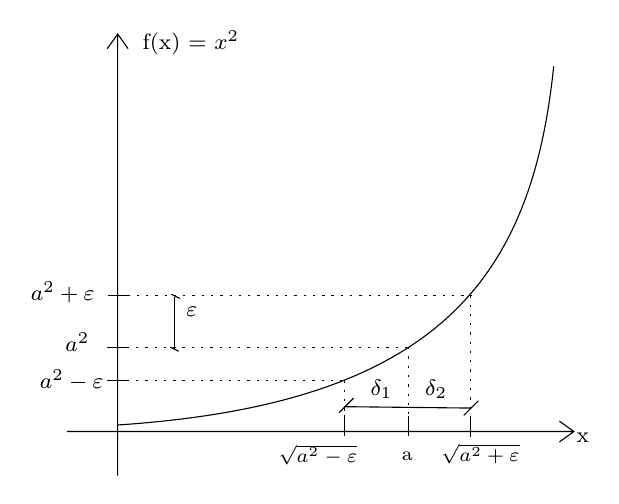
\begin{tikzpicture}[x=0.75pt,y=0.75pt,xscale=1,yscale=-1]
%uncomment if require: \path (0,299); %set diagram left start at 0, and has height of 299

%Shape: Axis 2D [id:dp3867480510801924] 
\draw  (186,243.98) -- (430.25,243.98)(210.43,52.5) -- (210.43,265.25) (423.25,238.98) -- (430.25,243.98) -- (423.25,248.98) (205.43,59.5) -- (210.43,52.5) -- (215.43,59.5)  ;
%Curve Lines [id:da24927309818628096] 
\draw    (210.43,240.83) .. controls (365.25,230.5) and (410,170) .. (420.5,68) ;
%Straight Lines [id:da573006633747857] 
\draw    (319.83,236) -- (319.83,246) ;
%Straight Lines [id:da48587909596300394] 
\draw    (380.5,236.67) -- (380.5,246.67) ;
%Straight Lines [id:da35466595178926763] 
\draw    (350.5,236.33) -- (350.5,246.33) ;
%Straight Lines [id:da5309416704381682] 
\draw    (214.83,219.33) -- (205.5,219.33) ;
%Straight Lines [id:da6214998288582192] 
\draw    (214.83,203.33) -- (206.83,203.33) -- (205.5,203.33) ;
%Straight Lines [id:da4810028574837353] 
\draw  [dash pattern={on 0.84pt off 2.51pt}]  (350.5,203.33) -- (350.5,236.33) ;
%Straight Lines [id:da4705268726888807] 
\draw  [dash pattern={on 0.84pt off 2.51pt}]  (214.83,219.33) -- (319.83,219.33) ;
%Straight Lines [id:da9900384690327877] 
\draw  [dash pattern={on 0.84pt off 2.51pt}]  (214.83,203.33) -- (350.5,203.33) ;
%Straight Lines [id:da90584733514422] 
\draw  [dash pattern={on 0.84pt off 2.51pt}]  (319.83,219.33) -- (319.83,236) ;
%Straight Lines [id:da8622465254367506] 
\draw  [dash pattern={on 0.84pt off 2.51pt}]  (380.5,178.33) -- (380.5,236.67) ;
%Straight Lines [id:da7681520132739281] 
\draw  [dash pattern={on 0.84pt off 2.51pt}]  (215.17,178.33) -- (380.5,178.33) ;
%Straight Lines [id:da8986518473983509] 
\draw    (215.17,178.33) -- (207.17,178.33) -- (205.83,178.33) ;
%Straight Lines [id:da5023958831241888] 
\draw    (319.5,232) -- (380.17,232.67) ;
%Straight Lines [id:da0905257915628539] 
\draw    (324.17,227.83) -- (317.17,234.83) ;
%Straight Lines [id:da7457981817486141] 
\draw    (384.17,229.17) -- (377.17,236.17) ;
%Straight Lines [id:da3169723653079166] 
\draw    (237.73,179.18) -- (237.73,204.1) ;
%Straight Lines [id:da969509824391011] 
\draw    (240.3,179.84) -- (236.25,177.84) ;
%Straight Lines [id:da40513119782948515] 
\draw    (239.83,205.32) -- (235.78,203.31) ;

% Text Node
\draw (221.17,49.67) node [anchor=north west][inner sep=0.75pt]  [font=\footnotesize] [align=left] {f(x) = $x^2$};
% Text Node
\draw (167.33,170.67) node [anchor=north west][inner sep=0.75pt]  [font=\footnotesize] [align=left] {$a^2 + \varepsilon$};
% Text Node
\draw (171.67,213) node [anchor=north west][inner sep=0.75pt]  [font=\footnotesize] [align=left] {$a^2 - \varepsilon$};
% Text Node
\draw (184,195) node [anchor=north west][inner sep=0.75pt]  [font=\footnotesize] [align=left] {$a^2$};
% Text Node
\draw (286.67,249) node [anchor=north west][inner sep=0.75pt]  [font=\scriptsize] [align=left] {$\sqrt{a^2 - \varepsilon}$};
% Text Node
\draw (365,248.67) node [anchor=north west][inner sep=0.75pt]  [font=\scriptsize] [align=left] {$\sqrt{a^2 + \varepsilon}$};
% Text Node
\draw (346,252.67) node [anchor=north west][inner sep=0.75pt]  [font=\scriptsize] [align=left] {a};
% Text Node
\draw (331,218) node [anchor=north west][inner sep=0.75pt]  [font=\footnotesize] [align=left] {$\delta_1$};
% Text Node
\draw (357.33,218) node [anchor=north west][inner sep=0.75pt]  [font=\footnotesize] [align=left] {$\delta_2$};
% Text Node
\draw (242.3,182.84) node [anchor=north west][inner sep=0.75pt]  [font=\footnotesize] [align=left] {$\varepsilon$};
% Text Node
\draw (430.33,243.33) node [anchor=north west][inner sep=0.75pt]  [font=\footnotesize] [align=left] {x};

\end{tikzpicture}
\end{center}
\section{Exercícios}
\subsection{Exercício 1:}
Nicole Oresme (1320–1382) foi um clérigo e matemático francês associado à Universidade de Paris, na Baixa Idade Média. (Katz, p. 392). Oresme determinou o espaço total percorrido por um móvel com velocidade variável, supondo que na primeira metade do tempo a velocidade é 1, no próximo quarto igual a 2, etc. (Katz, p. 398). Portanto, o cálculo equivale a determinar a soma da série:
\[
r_n = \frac{1}{2}\cdot1 + \frac{1}{4} \cdot 2 + \frac{1}{8} \cdot 3 + \dots + \frac{1}{2^n} \cdot n + \dots
\]

Ou seja,\hspace{0.2cm} \(r_n = \sum_{k=1}^{n} k \cdot a^k,\) \hspace{0.2cm} onde \( a = \frac{1}{2} \).\\

\begin{enumerate}
    \item[1.] Determine o valor de \( r_n \) em função de \( a \).
    \item[2.] Calcule o valor do limite \( \lim_{n \to \infty} r_n \), no caso \( |a| < 1 \).
\end{enumerate}
\textit{\textbf{Resolução:}}\\
\textbf{1)}
\[
r_n = \sum_{k=1}^{n} k a^k
\]
Reescrevendo:
\[
r_n = a \sum_{k=1}^{n} k a^{k-1}
\]
Seguindo a sugestão:
\[r_n=a\cdot\frac{-(n+1)a^n\cdot(1-a)+(1-a^{n+1})}{(1-a)^2}\]
\[=a\cdot\frac{1-a^{n+1}+(n+1)a^{n+1}-n\cdot a^n-a^n}{(1-a)^2}\]
\[=a\cdot\frac{1-a^{n+1}+n\cdot a^{n+1}+a^{n+1}-n\cdot a^n-a^n}{(1-a)^2}\]
\[=a\cdot\frac{1-a^n-n\cdot a^n(1-a)}{(1-a)^2}\]
Portanto:
\[r_n = \frac{a(1 - a^n)}{(1 - a)^2}-\frac{a\cdot n\cdot a^n}{1-a}\]
\vspace{1cm}\\
\textbf{2)}

Sabe-se que quando \( |a| < 1 \), \(\displaystyle \lim_{n \to \infty}a^n=0\).
\vspace{0.2cm}\\
Então, basta provar que \(\displaystyle \lim_{n \to \infty}n\cdot a^n=0\):

\[
\lim_{n \to \infty} n \cdot a^n = \lim_{n \to \infty} \frac{n}{a^{-n}}=\frac{\infty}{\infty}.
\]

Aplicando a regra de L'Hôpital:

\[\lim_{n\to\infty}\frac{n}{a^{-n}}=\lim_{n\to\infty}\frac{1}{-n\cdot\ln(a)\cdot a^{-n}}=\lim_{n\to\infty}\frac{a^n}{-n\cdot\ln(a)}\]

Como o numerador cresce muito mais rápido que o denominador, o limite será 0:
\[\lim_{n \to \infty} n \cdot a^n = 0.\]

Portanto:
\[\lim_{n\to\infty}r_n=\displaystyle\lim_{n\to\infty}\left(\frac{a(1-a^n)}{(1-a)^2}-\frac{a\cdot n\cdot a^n}{1-a}\right)\Rightarrow\lim_{n\to\infty}r_n=\frac{a}{(1-a)^2}\]

\newpage
\subsection{Execício 2:}
Calcule as 100 primeiras casas decimais de \(\pi\) usando a fórmula de Machin original, ou seja,

\[
\frac{\pi}{4} = 4 \cdot \arctan\left(\frac{1}{5}\right) - \arctan\left(\frac{1}{239}\right)
\]

Para isso, implemente o código em alguma linguagem de programação com precisão arbitrária, por exemplo Python.\\

\textit{\textbf{Resolução:}}

\begin{lstlisting}[language=Python, caption=Implementação do cálculo em Python]
from mpmath import mp

# calcula as 100 casas decimais
mp.dps = 100

# formula de Machin
pi = 4 * (4 * mp.atan(1/5) - mp.atan(1/239))

print(pi)
\end{lstlisting}
O valor de \(\pi\) com 100 casas decimais é:

\(
\pi \approx \textcolor{red}{3.141592653589793}2384626433832795028841971693993751058209749445923078164
\)
\(06286208998628034825342117068.\)

\newpage
\subsection{Exercício 3}
Calcule as casas decimais de \(\pi\) quebrando algum recorde histórico pós-1949. Por exemplo, 2.037 casas obtidas pelo ENIAC em setembro de 1949. Para tanto, use as fórmulas:

\[
\frac{\pi}{4} = 12 \cdot \arctan\left(\frac{1}{49}\right) + 32 \cdot \arctan\left(\frac{1}{57}\right) - 5 \cdot \arctan\left(\frac{1}{239}\right) + 12 \cdot \arctan\left(\frac{1}{110443}\right)
\]
(K. Takano, 1982)

\[
\frac{\pi}{4} = 44 \cdot \arctan\left(\frac{1}{57}\right) + 7 \cdot \arctan\left(\frac{1}{239}\right) - 12 \cdot \arctan\left(\frac{1}{682}\right) + 24 \cdot \arctan\left(\frac{1}{12943}\right)
\]
(F.C.M. Størmer, 1896)

\vspace{0.2cm}
Usando a segunda fórmula para verificar o resultado obtido pela primeira.

\textit{\textbf{Resolução:}}
Implementando o código em Python, como no exercício anterior:

\begin{lstlisting}[language=Python, caption=Calculando 2100 casas decimais de PI]
from mpmath import mp

# calcula as 2100 casas decimais
mp.dps = 2100

# formula de K. Takano 
pi_takano = 4 * (12 * mp.atan(1/49) + 32 * mp.atan(1/57) - 5 * mp.atan(1/239) + 12 * mp.atan(1/110443))

# formula de F.C.M. Stormer
pi_stormer = 4 * (44 * mp.atan(1/57) + 7 * mp.atan(1/239) - 12 * mp.atan(1/682) + 24 * mp.atan(1/12943))

print("Valor de pi usando K. Takano: ", pi_takano)
print("Valor de pi usando F.C.M. Stormer: ", pi_stormer)
\end{lstlisting}

O valor de \(\pi\) com 2100 casas decimais usando a fórmula de \textbf{K. Takano} é: 
\[\textcolor{red}{3.1415926535897930}42929663938552056294267246929749682\cdots\]

O valor de \(\pi\) com 2100 casas decimais usando a fórmula de \textbf{F.C.M. Størmer} é: 
\[\textcolor{red}{3.1415926535897930}56924425796766148906536443774591942\cdots\]
Assim, vemos que o resultado obtido através da segunda fórmula coincide com o da primeira até as 16 primeiras casas decimais, divergindo posteriormente.\\

Comparando também com o resultado obtido pela Fórmula de Machin original (1706):
\[\textcolor{red}{3.141592653589793}238462643383279502884197169399375105\cdots\]
Vemos que do resultado dela coincidem apenas as 15 primeiras casas decimais quando comparadas com os resultados acima.

\end{document}
